\documentclass[12pt,a4paper]{report}

%% Language and font encodings
\usepackage[english]{babel}
\usepackage[utf8]{inputenc}
\usepackage[T1]{fontenc}
\usepackage{indentfirst}
\usepackage{csquotes}
\usepackage{textcomp}

%% Sets page size and margins
\usepackage[a4paper,top=3cm,bottom=2cm,left=3cm,right=3cm,marginparwidth=1.75cm]{geometry}

%% Useful packages
\usepackage{graphicx}
\usepackage{amsmath}
\usepackage{subcaption}
\usepackage[colorinlistoftodos]{todonotes}
\usepackage[colorlinks=true, allcolors=blue]{hyperref}
\usepackage{multirow}


%% Applying settings

\begin{document}
\begin{titlepage}
\title{Flexible Bio-metric Sensors}
\centering
{\scshape Carleton University \par}
\vspace{1cm}
{\scshape Fourth Year Project Final Report\par}
\vspace{1.5cm}
{\huge\bfseries Flexible Biometric Sensors\par}
\vspace{2cm}
   
{\scshape\Large Thermal Sensor Design and Testing\par}   
    By
    
{\Large\itshape Brendan Armstrong\par}
    (100921048)
    \vfill
    Partners
    
    {\large\itshape Thomas Young \par}
    (100998208)
    
    {\large\itshape Maharshi Gurjar\par}
    (101094330)
    
    {\large\itshape Cameron Toswell\par}
    (101037032)
    
    {\large\itshape Tariq Aboushaer\par}
    (101064544)
    
\vfill
supervised by\par
Dr.~Ravi \textsc{Prakash}

\vfill

%% Bottom of the page
{\large \today\par}
\end{titlepage}

\begin{abstract}
    Sensor Node Design is an important part of electronics and automation sector. This project group decided to make a sensor node with a thermal sensor, perspiration sensor, and blood pressure sensor. \par
    This report will dedicate its attention to the design and testing of the first iteration of thermal sensors in the sensor node.
    \par
    An RTD positive temperature coefficient thermistor is designed in a serpentine fashion and fabricated on a silicon wafer. Two groups of these thermal sensors were tested, the Large sensors of size ($1cm^2$) and the small sensors of size ($0.5cm^2$). The sensors were made of chromium and calibrated with a room temperature of 12\textcelsius{} and a temperature of 33\textcelsius{} which was produced by a hair dryer blowing on them. The calibrated sensors were then used to measure body temperature of both the wrist and the underarm to test their accuracy and precision. The sensors were accurate to the calibration thermometer used and precise to within 0.5\textcelsius{}. There is a systemic error of approximately 15\textcelsius{} in this first iteration due to the calibration thermometer being of lower quality.
\end{abstract}


\newpage
\vspace*{2in}
\section*{Acknowledgements}
this project was done in difficult times and I would like to thank all of those who made it possible. Please allow me to officially extend my gratitude towards the following people.

\begin{enumerate}
    \item[] Dr. Ravi Prakash - For supervision in these trying times
    \item[] Nagui Mikhail - For providing equipment and components
    \item[] Dr Tom Smy \& Dr Shulabh Gupta - For providing feedback on our presentation
    \item[] Mounia \& Ivan - For help with mask fabrication
    \item[] Rob, Angela, \& Rodney - For fabricating our sensors for us
    \item[] Dr. Sizi Bebe - For creating the pressure sensor with PVDF
\end{enumerate}

I would also like to thank my group members who were willing to work with what we were given from start to finish. This was a nice way to finish my degree.



\newpage
\tableofcontents
\newpage
\listoftables
\begingroup
\let\clearpage\relax
\listoffigures
\endgroup

\newpage

\renewcommand{\thesection}{\arabic{section}}




%%%%%%%%%%%%%%%%%%%%%%%%%%%%%%%%%%%%%%%%%%%%%%%%%%%%%%%%%%%%%
\section{Introduction}
%%%%%%%%%%%%%%%%%%%%%%%%%%%%%%%%%%%%%%%%%%%%%%%%%%%%%%%%%%%%%

\subsection{Overview/Background}

The purpose of this project was to create a bio metric sensor node that could be worn. The information collected from the sensor node would then be transmitted via Bluetooth to a phone app such that the wearer could then read the data. \par

The sensor node would be comprised of a temperature sensor, a perspiration sensor, and a blood pressure sensor. These metrics would allow for the inference of health abnormalities and alert the user prior to experiencing physical symptoms.\par

The circumstances at the time of this project made it difficult to carry the teams dream to fruition. Throughout the second half of the semester, we had major setbacks and time delays and as a result, only a preliminary set of sensors was fabricated and used to read data while tethered to the computer. The Data was then processed, the sensors were calibrated, and only the perspiration and temperature sensors were fully integrated into one system. In a cruel stroke of fate, these delays were caused by the very source of our motivation, the pandemic of 2020.

\subsection{Motives/Significance}

Many projects take their motivation from the state of the environment in which they were performed. This project is much the same, only at the time this project was being formulated, a world-wide pandemic was dominating our lives. COVID-19 is a terrifying virus not just because of its efficacy, but because it's asymptomatic transmission. The host of the virus does not even know they are infected and will spread the disease for days before they present physical symptoms, if they develop symptoms at all. \par

It is for this reason that our group has decided on measuring health parameters so that we may detect early symptoms of illnesses that would have otherwise been unnoticed. Another use of these wearable sensors would be fitness monitoring, we could have stored the wearers data in the phone app and processed it to score general fitness and activity levels. This would be similar to currently available devices like the fitbit.

\subsection{Design Objectives}

The sensor node needed to be able to be worn around the users arm. This would be done with a flexible material. This means that it needed to be comfortable and have the potential to be stylish. There would need to be an on-board power supply as well as a processing and transmission module to send data to the phone app. The phone app would need the ability to display information, and since our original idea was to process the data using the phones processor, that is where all of out back end capabilities would come into play. Should the user show signs of health degradation, the phone app should alert the user.

\subsection{Design Specifications}

We had decided that the flexible material which would contain the wearable circuitry would be kapton, a polyimide film that can remain stable at temperatures from $-269$ \textcelsius{} up to $400$ \textcelsius{}. This temperature range is suitable because our target range is between 20-40 \textcelsius{}. The perspiration sensor was supposed to sense moister from sweat generated by the user. We opted for a capacitive sensor with interdigitated electrodes. The blood pressure sensor needed to sense small changes in pressure caused by the pulse of the users artery. In order to achieve this, we had decided on PVDF, a piezoelectric polymer which generates voltage when the structure is deformed.\par
The thermal sensor was decided to be a positive temperature coefficient thermistor and will be discussed at great length in this report.

\subsection{Relevant Publications}

Since this project was one of electrical nature, the first source of information i choose to draw from was Sedra/Smith \cite{Sedra2010}. This reference contains all the circuit knowledge that I needed and came in use when I was designing the differential amplifier for signal processing, shown in fig \ref{fig:ConditioningCircuit}. One of the largest problem that I had was trying to filter the signal output of my initial circuit in fig \ref{fig:InitialCuircuit}. I will discuss the challenges I had with the conditioning circuit in later sections. Other resources include the journal articles which our professor sent. I used two of the journal articles, the 2018 article \cite{Sensors2018} which goes over a four in one sensor module for the purposes of monitoring proton exchange in fuel cells. And the 2016 article \cite{Nature2016} which takes an in depth look at in situ perspiration analysis. In order to get the values for the metals to use in fabrication of the sensors I used the engineers toolbox website \cite{Etool}.
\par

In order to get the prefabricated microprocessor to work I used documentation from Adafruit \cite{ADA} to get it to work with the arduino integrated development environment. I also spent a great deal of time trying to find a way to extract the data from the serial readout of the FLORA. This is where the free software that I found comes into play. CoolTerm is is software that I got from \cite{CoolTerm}, it was made by a man named Roger Meier who is an electrical engineer operating out of Florida. CoolTerm watches serial ports on your PC and duplicates it and gives you the option to print the output to a txt file.

%%%%%%%%%%%%%%%%%%%%%%%%%%%%%%%%%%%%%%%%%%%%%%%%%%%%%%%%%%%%%
\newpage
\section{Professional Considerations}
%%%%%%%%%%%%%%%%%%%%%%%%%%%%%%%%%%%%%%%%%%%%%%%%%%%%%%%%%%%%%


\subsection{Engineering Professionalism}

    Engineer is a protected term meaning that you cannot claim to be an engineer without a license. Falsely claiming you are an engineer could be a fine up to \$25,000 as it is a protected title. The purpose of professional engineering is to preserve the safeguarding of life, health, property, economic interest, the public welfare or the environment. An organization must have at least one professional engineer who will take responsibility for engineering and be insured against professional liability. A regulated professions primary purpose is quality assurance. The licensing first started in 1896 to ensure the professional safety of engineering. There are twelve engineering regulators across Canada. The purpose of engineers Canada is to serve the regulators, promote and maintain the interests, honor, and integrity of engineering in Canada. There are ten tenants to govern the regulators; 
    
    \begin{enumerate}
        \item Accrediting undergraduate engineering programs.
        \item Facilitating and fostering working relationships between and among the regulators.
        \item Providing services and tools that enable the assessment of engineering qualifications, foster excellence in engineering practice and regulation, and facilitate mobility of practitioners within Canada.
        \item Offering national programs.
        \item Advocating to the federal government.
        \item Actively monitoring, researching, and advising on changes and advances that impact the Canadian regulatory environment and the engineering profession.
        \item Managing risks and opportunities associated with mobility of work and practitioners internationally.
        \item Fostering recognition of the value and contribution of the profession to society and sparking interest in the next generation of professionals.
        \item Promoting diversity and inclusively in the profession that reflects Canadian society.
        \item Protecting any word(s), mark, design, slogan, or logo, or any literary, or other work, as the case may be, pertaining to the engineering profession or to its objects.
    \end{enumerate}
    
    Engineers Canada maintains relationships with the Canadian government to ensure engineers can work together with the country when making policies. The government will then publishes statements on public positions related to engineering. Engineers Canada also has national position statements on various topics.

\par

    In this section the requirements to become and engineer will be discussed, with an emphasis on health and safety at work as well as the code of ethics and protection of public interests.




    \subsubsection{Professional certification requirements}
    
   
    
    The accreditation board was established in 1965 and accredits engineering programs that meet the requirements. The qualifications board promotes mobility, consistent practices and shared programs. They also help international engineers who want to work in Canada.\par
    
    Licensure is the mark of a professional. Any act of designing, composing, evaluation, advising, reporting, directing, or supervising where life, health, property, or public welfare is concerned that requires the application of engineering principles requires a license. Many graduates believe that graduating allows them to call themselves engineer. However the license is what determines if you are an engineer. There are five categories for getting a license;
    
    \begin{enumerate}
        \item Academics
        \item Work Experience
        \item Language
        \item Good Character
        \item Professionalism and Ethics
    \end{enumerate}
    
    In Canada, engineers must be able to communicate in English or French.  Licensing requirements include an acceptable engineering education or a practical examination. You must have good character and references from a minimum of one professional engineer. You must take a professional practice examination which is about 3 hours long. Ethics is important as engineers are professional representatives for all engineers.\par
    
    Professional engineers Ontario (PEO) is a regulatory body that governs engineering in Ontario where there are over 80,000 engineers. The head office is in Toronto at young and Shepard. PEO is self-regulating and sets standards for Ontario. Formed in 1922, before this, engineers did not practice to a set standard and instead engineered to their own standards. The regulation of PEO happens through three steps, admissions, enforcement, and discipline. They have the power to give licenses and take them away. Similar associations are found in other provinces however PEO is the regulatory body in Ontario. There are about 190,000 engineers in Canada. Engineers Canada is the umbrella organization for the national standards. Those who are licensed in one province are able to move to other provinces. 
    \par
    There are two basic types of law, statutory law created by legislative bodies, and common law, created from precedent. An Act is the primary law governing some issue of public interest. The professional engineers act creates a controlled activity of professional engineering; it establishes PEO as the authority. Regulations are the secondary level of laws. Power to make regulations is delegated to the ministries that govern the areas of interest. PEO has the power to grant licenses. There are two regulations under the professional engineers act. Regulation 941 and regulation 260/08, 941 govern elections and code of ethics.  260/08 governs professional standards and inspections.
 
    
    \subsubsection{Health and safety at work}
    
    Engineers are required to safeguard life, health, and property. Engineers have a duty to act with fairness and loyalty, fidelity to public needs, and devotion to public good. OHSA talks about your rights and responsibility of workers and employers. The internal responsibility system talks about a joint health and safety committee and health and safety representatives. The ministry of labour is the enforcement body for the health and safety of workplaces. The ministry of labour inspectors do not need warrants to enter and inspect a workplace. Individuals can be fined up to \$25,000 per charge and corporations can be fined up to \$500,000 for each charge. The criminal code changed in 1992 due to an explosion at a mine where the officers on site could have reported it but did not.  Bill C-45 states that any officer is under the legal duty to take reasonable steps to prevent harm arising to workers. Employers must make sure they inform workers about dangers and how to avoid them. Constructors are responsible for ensuring the safety for all employees on that project. Workers must obey safety procedures and report hazards to the higher-ups. \par
    
    Hazards can take two forms, acute and chronic. Acute hazards are immediate dangers. Chronic hazards are due to long lasting hazards. A third category of hazards is latent, where the effects appear much later after the hazard has happened. Illnesses are caused by exposure to a harmful substance. Inhalation, ingestion, skin absorption or injection is the primary means that harmful substances enter our body. All dangers that are present in the workplace must be considered and a strategy for preventing them created. Hazards can be controlled at the source, along the path, and at the worker. If you cannot control the source of the hazard, you can control the hazard along the path to the worker. If that is not possible then the hazard can be controlled at the worker but this is not recommended because every worker is unique and variations will occur. \par
    
    Pre start health and safety review (PHSR) is in the design work of an engineer. There are many aspects to the PHSR for which a professional engineer is responsible. The PHSR must be completed prior to the workplace functioning and the report should be kept on site. Engineers are responsible for arranging the compliance of apparatus, structures or protective elements.
    
    
    
    \subsubsection{Code of ethics and protection of public interest}
    
    Ethics is an activity we engage in every time we ask the question “what should I do”. Ethics is concerned with taking actions that will create positive results in one’s life or the lives of others. The four major ethical theories are; Virtue based ethics, Rights based ethics, Duty based ethics, and consequence based ethics.
    \par
    Virtue based ethics was formed from Aristotle and means discerning and promoting the proper goals. Paying attention to how things work and discerning their inner structure. A virtue is a cultivated habit, a formation of character. The limitations of virtue based ethics involve the reliance on strangers following rules and not character evaluations.\par
    
    Rights based ethics of John Locke revolves around the rejection of authority. The goal is to allow all persons full liberty and full participation in society. When living in society we use reason to establish social contracts to direct how we live. Rights based ethics divides rights into public and private spheres. Public spheres are enforced by courts of law. The private realm establishes individual rights for private affairs like belief system. \par
    
    Duty based ethics of Immanuel Kant was established around the obligations of individual in a society. Personal conviction and rational autonomy are the primary focuses of duty based ethics. One should act in accordance to principles that must be applicable to all persons, not just ourselves, act onto others as you want others to act to you. The limitations of duty based ethics are conflicting obligations and overemphasis on the law.  \par
    
    Consequence based ethics or Utilitarian ethics was created by John Stuart Mill. It was created because a standard was necessary to compare ethics. Humans naturally pursue their own happiness. Sometimes what is good for an individual isn’t good for the group, Utilitarian ethics judges actions based on the overall good it accomplishes. \par
    
    No one model is sufficient, a combination of these ethical models is necessary. When deliberation is performed an activity in ethical dynamics is taking place to discover the best course of action. The framework for ethical deliberation is aims at understanding the overall goal of ethics. The diagnostic loop is an effective tool for ethical deliberation, exploring the situation, verifying it, deciding on what to do then paying attention to the results. \par
    
    
    Regulation 941 governs the ethics of engineering in Ontario. The core ethics of engineering consists of three categories, Professional misconduct, Code of ethics, and whistleblowing. 
    \par
    
    Professional misconduct is being convicted of an offence that relates to the practice of professional engineering. Acting in a negligent manner includes positive actions and omissions. \par
    
    Negligence can be divided into three elements. A failure to act when it will impact another person or the public, not fulfilling standards or causing property damage are all elements of negligence.
    \par
    
    Commissions is performing work which you are not licensed to do. Omissions are not making reasonable provisions during the course of your work. The punishments for violating professional misconduct range from revocation of the license and suspension to fining. Publishing the details of the violation publicly is also a possibility and this is particularly damaging. \par
    
    The five primary categories are the obligations to;
    
    \begin{enumerate}
        \item The Public
        \item The Clients
        \item The Profession
        \item The Employer
        \item Everyone Else
    \end{enumerate}
    
    Obligations to the client include conflicts of interest. If you have a bias to a project that will affect the outcome, this must be disclosed. Obligations to professionals includes enhancing the public regard for professional engineering. You must discourage actions that will diminish the public’s image of engineers. You have an obligation to cooperate with other professionals. Giving proper credit or compensation for others work is in the obligation to other professionals.  You must act faithfully to your client as an agent and trustee of information. Obligations to everyone include having high ideals of honor and integrity.
    \par
    
    Failure to make reasonable provisions for the safeguarding of life, health, or property of a person or public is a violation of the code of ethics. You owe fairness and loyalty to your client, however if the clients actions violate the code of ethics you have the option for whistleblowing. This option will severely effect your future as you will be known as a whistleblower.
    
    
\subsection{Impact of Engineering on Society}

 Engineering’s impact on society can be easily seen in just the past 100 years, power grids and cell phones are just part of the importance. The first duty of the engineer is public safety. Some of the earliest engineers were the ancient Egyptian and Mesopotamian engineers who built pyramids. The only tools at their disposal were primitive, and the mathematical tools we have like the Pythagorean Theorem were not yet invented. Greek engineers were known as architekton, a master of the practical arts. Roman engineers were masters of project management. They built the famous aqueducts, the pantheon, and the colosseum. Leonardo da Vinci was a multi-talented engineer in the Italian renaissance who predicted the helicopter and tank. Early engineers made huge impacts on everyday life and will continue to do so in the future. \par

 Regarding sustainable designs, Safety measures, and economic implications, in this section, the role that engineers play in society and the responsibilities associated with the position will be discussed. 

    \subsubsection{Place of engineering in society}
    
    The Canadian parliament passed an act in 1887, to include civil engineers into the engineering profession. This was the start of the professional engineering in Canada. Since then, many Canadian engineers have done great work. Elsie MacGill was the first Canadian Woman to earn a degree in Electrical engineering in 1927. She was the first woman in North America to earn a degree in aeronautical engineering. Canada has had some terrible failures unfortunately. The Quebec Bridge collapsed twice killing many people. The first meal cooked with electricity in the world was cooked in Ottawa. \par
    
    Engineering in our society requires people who are diligent enough to take even small factors into consideration. For example, the Tacoma narrows bridge was negligently designed such that the oscillations produced from the wind rolling past it excited the bridges resonant frequency. This led the famous collapse, not only causing massive economic damage, but also damage to the engineers reputation.
    
    
    
    \subsubsection{Sustainable design; life-cycle planning}
    
    Engineers are bound to a code of ethics which extends to the environment. Engineers take a cradle to grave approach when designing to analyze the full life cycle of a product. Environment Canada monitors the environment.  The Canadian environmental protection act (CEPA) was created in 1999. The act prevents pollution and elimination of bio accumulative toxins. Waste must be disposed of properly because it could affect the environment.  Owners of substances are strictly liable for restoration or reparation of public sites where damage has been caused.\par
    
    
    Sustainability must be quantifiable. Greenwashing is marketing products as sustainable when they aren’t really sustainable. Bottled water is about 2000 times more energy expensive than tap water, making it not very green. Sustainability concerns the actions taken by present persons that will not impact future persons. Economic sustainability allows for future persons to have wealth. Social sustainability is the least well defined but consists of 5 parts;
    
    \begin{enumerate}
        \item Quality of Life
        \item Equity
        \item Diversity
        \item Social Cohesion
        \item Democracy
    \end{enumerate}
    
    Environmental impact is equal to the product of the population, affluence, and technology. The ecological footprint is the fraction of resources allocated to a population. The current carrying capacity of earth is about 3-13 billion. 
    \par
    
    The first challenge in sustainability is limited temporal scope. We don’t have a far enough view into the future to recognize costs. A limited spatial scope is a problem as well, as we don’t look at what happens far enough around us. People often don’t think far beyond themselves which makes it hard to improve sustainability. An example of this is the protesting of green power turbines near them. The tragedy of the commons is a problem which states that other people will exploit resources so if you don’t exploit them, you will lose. Jevons paradox states that if you make a product more sustainable, people will just use it more. We cannot modify human behavior directly, but if we make the path that humans take the most efficient ones, then we can get ahead.
    \par
    Quantifying sustainability is important to improving it. Assign value to externalities in the process of creation. Assess the impact of a products life cycle. And keep in mind the material flow in the process. Looking at the whole life cycle of a project will reveal the true costs that will be incurred. Putting sustainability into practice involves modifying technology. We can make the world better by using more efficient materials, less energy, and overall make technology better for the world. Sustainability can improve by designing products to last longer. Bio-mimicry is a useful strategy for sustainability by imitating nature. 
    
    \subsubsection{Interactions(with society and stakeholders)}
    
    The industrial revolution and mechanical engineering started in Great Britain and spread rapidly. James Watt created the steam engine in 1765 and brought forth the ability to get power without relying on falling water. He created this engine in order to pump water out of a coal mine to extract more coal. In the 19th century, electrical engineering bloomed with scientists like Ohm, Faraday, Maxwell, and Siemens. There was a battle between Edison and Tesla for using DC current and AC current respectively. Edison was particularly petty, He even shocked animals in a public forum to show people that AC was dangerous, But Tesla still won and we use AC today. 
    \par
    Not only do engineers need to design things to work, but they also need to design things to work when the most "creative" people are using the things. Designing solutions to problems must take society into account.
    
    \subsubsection{Health, safety, and risk}
    
    Engineering can have an impact on environmental issues as well as health and safety issues. It is because of this that government regulations have come in to set standards.\par
    
    Within the province of Ontario there are environmental statues that protect the environment like the green energy act. The Ontario environmental protection act (EPA) is the primary regulation in Ontario. The basic intent is to prohibit the emissions of negative environmental substances.  Approval from the EPA is required for any discharge from stacks, wastewater or waste deposits on land. There is a requirement for the best available economically viable technology. Ontario also has a secondary tier of approvals called the environmental activity and sector registry (EASR). It is intended to govern the lower risk activities including heating systems and power systems. The EASR required a registration of low risk activities, and getting approval or permit for renewable energy generation. \par
    
    The EPA has regulations around spills and contamination. In the event of a spill or contamination, you are obligated to notify the spill action center. You are required to do everything practicable to clean up spills. Maximum fines for corporations are up to 10 million and individuals can be imprisoned for up to 5 years.\par
    
    The green energy act was enacted to encourage new green energy technology development. Ontario has programs where costs can be partially reimbursed to companies that install renewable energy. Only British Columbia and Quebec have carbon taxes based on how much energy is used. Purchasers of companies acquire all assets and liabilities including past environmental issues. 
    
    
    
    
\subsection{Economics \& Project Management}

For engineering projects to be successful, a manager must allocate resources where they are the most effective. In this section, I will be talking about the time value of money, depreciation, amortization, and taxes. As well I will be talking about risk and time management.

    \subsubsection{Engineering economics}
    
    Effective resource management is crucial for any project to be successful. The first step to realizing how to allocate resources effectively is to understand the time value of money. Money itself depreciates with value every day it is held as FIAT currency, so a good way to grow money is to trade money today for something that will grow with value over time. This is why money is thought to have a "time value". For example, the 'S\&P 500'(SPY) has historically had a growth of 7\%-8\% per year growth, when compared to historical inflation at approximately 2\% this means shares of SPY grow in value at a rate of 5\%-6\% per year. This means that money is made simply by owning an item of value. an engineering project can be thought of in the same way but with more growth and decay parameters.\par
    There are other factors which cause resources to experience the same fluctuations in value. Taxes are a source of a lot of creativity when it comes to financial engineering. When a project successfully generates revenue, that money is taxes by the government. In order make more money, some of these taxes will need to be avoided. This can be done through amortization of assets, which is the process of paying off a large purchase over many tax intervals. Doing this, the value of the payments can be deducted from taxable income and more resources can be used for the project.\par
    
    Money can also be harvested from the expensive equipment at the end of their life for a salvage value. In addition to the value of assets, a good manager also considers the value of the team at their disposal. This is where risk and change management comes into play
    
    \subsubsection{Risk and change management}
    
    In engineering challenges, there are risks and there are fixed parameters. Fixed parameters are things like prices, interest rates, and cash flows. Risk comes with uncertain outcomes. In order to properly assess the risk of a project, a sensitivity analysis will need to be preformed. The first step is to make a break even analysis, which is used to assess the effect of changes in project parameters one at a time. A good manager will also understand the probabilities of events happening and how to account for them in an economic analysis. These factors will then be used to make a decision tree.\par
    
    The break even analysis is the process of varying one parameter of the project at a time to find the break even point, the point at which cost equals revenue. When preforming break even analysis, one must consider how many projects are available and if they are mutually exclusive, the best choice for which projects to pursue will be a combination of interest rate, revenue, and initial investment.\par
    
    Obtaining the appropriate probabilities of events happening, and how to apply them to management decisions. A probability is found either through historical data for educated inference and can be applied as a weight to the outcome with which it is associated. After all outcomes and probabilities have been calculated, a decision tree can finally be made. \par
    
    There are four components of a decision tree;
    
    \begin{enumerate}
        \item  A decision node represents a decision to be made.
        \item  A chance node represents an event whose outcome is uncertain.
        \item  The branches connect nodes from left to right.
        \item  The leaves indicate the values, or payoffs.
    \end{enumerate}
    
    In this case, the leaves are at the end of the tree and typically the largest leaf is selected. This leaf is selected even if there is risk associated with it because the risk is factored in with the weight of the probability.
    
    \subsubsection{Individual and team work}
        \renewcommand{\theenumi}{\roman{enumi}}
        \begin{enumerate}
            \item Personal and group time management.
            \vspace{2mm}
            
            Different members of our group had different time schedules due to taking on multiple responsibilities for the duration of the project. But we made sure to meet twice a week. once with the professor and once on Saturday at 11:00am. Our meeting with the professor was Thursday for the first semester and moved to Wednesday for the second semester. Occasionally when deadlines were approaching, our group would hold a second meeting after the meeting with the professor in addition to the meeting on Saturday. Asynchronous communication was also heavily utilized by the group though our MS teams chat. \par
            
            As for my own personal schedule. The first semester was heavy for me in terms of class work. I was taking 4 other classes in addition to project so my work would fit whatever time i gave it. But the second semester was completely free for me. Project was the only obligation I had aside from my part time job as an emergency superintendent in my building, which rarely required my attention. I contribute my success in troubleshooting problems to this freedom. Since this was a remote project, I was mostly required to solve problems with testing or equipment on my own. Although I received some help whenever I really needed it, it was difficult to email people for advice on trivial things. Since I had all the extra time, this was how i spent it. Eventually I sent the equipment to Thomas who then started to do his own testing. I was then able to focus on processing my data.
            
            \item Group culture, group dynamics
            \vspace{2mm}
            
            With the entire semester being online only, the group had an unusual dynamic. We established our roles early on in the project and kept in constant contact through MS teams. Through our shared displeasure at the situation we were able to come together and solve problems. When the testing equipment and older IDE's were delivered to our possession, there were days when we spent hours on voice/video chat trying to trouble shoot how we could read the old sensors. Not having any physical interaction with any of our members was weird for group cohesion. Maharshi was in charge of the conditioning circuit, but seemed distant and would only respond to the group when he was directly inquired. This led to me ultimately having to create my own low pass filter from my own research\cite{Sedra2010}. Tariq was eager to prove his worth but kept getting himself into situations, like moving to Saudi Arabia and contracting COVID, he even had a problem with his eye where he couldn't see for 2 weeks. Cameron was in Ottawa but his role was primarily software based so we didn't interact as a group often. A great deal of the MS teams private chat is Thomas and myself trying to troubleshoot problems. I feel that a lot of group members were worried about the amount of work that they could potentially put into the project not being enough to satisfy requirements. This ended up as a great source of strain in moments of high tension. But every time tensions flared up, we sorted it out and ultimately came through with a positive mental attitude.
            
            \newpage
            \item Leadership, initiative, and mentoring teammates
            \vspace{2mm}
            
            Since the beginning of the project, I wanted to move the meetings along the right path and make efficient use of our time. It was for this reason that I eventually became de-facto leader of the project. One of the problems was that this wasn't officially established until later in the project. There were times when i thought that group members should have been more active in the chat to give their input. But without a clear designation of leadership I feared it would sow discontent if I voiced that opinion. There were multiple moments where Tariq would come to me about project questions and concerns and I believe he saw me as the leader. Near the end of the project though, after the equipment was transferred, Thomas ended up taking on more responsibility in testing and helping Tariq get readings from his pressure sensor.
            
        \end{enumerate}

%%%%%%%%%%%%%%%%%%%%%%%%%%%%%%%%%%%%%%%%%%%%%%%%%%%%%%%%%%%%%
\newpage
\section{Theory \& Technique}
%%%%%%%%%%%%%%%%%%%%%%%%%%%%%%%%%%%%%%%%%%%%%%%%%%%%%%%%%%%%%
Now to refocus our sights on the primary topic of this report, the thermal sensor. My contribution to the project was the design and testing of the thermal sensor and in this section I will be discussing what this means. First I will asses the design options available for thermal sensors and consider the economic, social, environmental, and ethical impacts that these options have. I will then discuss the choice of thermal sensor made and go into detail about specific parameters of the design. After the final design has been revealed I will talk about the challenges of trying to test sensors in my home laboratory and how I managed to overcome these challenges to receive precise results.


\subsection{Alternative Design \& Assessment}

When considering Thermal sensors there are four types of sensors for consideration;
\renewcommand{\theenumi}{\Alph{enumi}}
\begin{enumerate}
    \item Thermocouple
    \item Semiconductor
    \item Negative Temperature Coefficient
    \item Positive Temperature Coefficient
\end{enumerate}

Each of these types of sensors has their advantages and disadvantages. When thinking about what type of thermal sensor to choose it would be prudent to keep in mind the criteria that need to be met. As stated in introduction, this sensor is intended to be a bio metric sensor that will be worn against the body to provide health measurements while being worn. The temperature sensor needs to measure temperatures accurately within the range of 20\textcelsius{} to 40\textcelsius{}. The physical sensor itself must be flexible enough to survive being fabricated on Kapton and survive though out its life cycle. The sensor must also be comfortable to wear against the skin for extended periods of time. The life cycle of the sensor was never a point of consideration for this project as our group did not reach the point of prototyping for consumption. Since this is the case it was assumed the life cycle would be the life of the user at approximately 80 to 100 years.\par

A thermocouple is a device which has two dissimilar metals electrically bonded to each other. As the two metals experience a temperature change, internal charge carriers migrate towards the metal with lower internal energy. This causes a voltage to be generated across them. This technology is widely used as an inexpensive method of temperature control and is versatile because it can also be used in reverse. If a voltage is passed through a thermocouple it can be arranged so that it will "pump" heat from one place to another, so it makes a good temperature control system as well as a temperature detector. The disadvantages of thermocouples are that they would be uncomfortable for the user to wear given their shape. this also needs a reference temperature that would remain stable, which is difficult to do because one of the temperatures would be body temperature and the reference would be atmospheric which is cyclic in nature and would not remain stable. The output of thermocouple is non linear in nature which would mean that more components would be necessary to process the signal.\par


Semiconductor based thermal sensors exploit the thermal response of semiconductors. As a semiconductor junction heats up, more charges are excited to the conduction band creating a temperature sensitive voltage vs current response. these sensors typically have a linear output from -40\textcelsius{} to 120\textcelsius{}. when manufactured en mass they are low cost and have good accuracy. Though the durability of the semiconductor material would be questionable when trying to apply them to a flexible material and read body temperature. The underlying material would be doped silicon or a similar ceramic material, so with repeated stress applied from flexing the arm band the sensor may break.\par

The next two categories of thermal sensors operate in the same fashion, they are the resistance temperature detector (RTD) thermal sensor. They operate by exploiting the temperature dependant change in  the electrical resistive properties of materials.\par

The first class mentioned in the list above is the negative temperature coefficient thermistor. this type of RTD decreases its resistance in response to an increase in temperature. This type of sensor is made from ceramics or polymer materials. The polymer version of this sensor could be suitable for this project as it would be flexible enough to survive use. However there is one fatal flaw with this type of sensor, the non-linearity of output response. This means that a larger processing circuit will be required to make it operate. This also means that the specialized polymer would be more expensive.\par

The final class of thermal sensor is the positive temperature coefficient RTD. This sensor increases in electrical resistance as the temperature of the material increases. This type of sensor is made of metals and has an accurate linear output within the range of -200\textcelsius{} to 600\textcelsius{}. This temperature range is ultimately dependant on the metal chosen and the substrate on which it rests. Since the sensor will be deposited on Kapton it will work for temperatures up to 400\textcelsius{}. The temperature characteristics may be overkill since they suitable to be used on the surface of Venus, but other factors make this type of sensor more attractive than the others. Because these sensors are made from cheaper metals, the cost is low and made lower if they can be manufactured en mass. These sensors will be made with metal deposition so the thin metal will not only be comfortable, but it will be able to survive the fatigue of being mounted on a flexible piece of active wear.\par

From an economic standpoint, depositing metal on Kapton seems to be the best place to start since the mask could be reused and the entire circuit could be printed on the polymer substrate. as for the environmental implications, Kapton as a polymer does end up in landfills along with other electronics frequently there is a great effort to develop new recycling techniques for this polyimide material. This technology does not change the social landscape so there would be no effect there. And the worst ethical argument one could make towards this technology is that of environmental waste.\par

With consideration of all of these arguments, the most effective thermal sensor for the purposes of this project is the Positive temperature coefficient RTD. In the next section the specifics of the design with this style of thermal sensor will be discussed.

   
\subsection{Chosen Design Details \& Verification}

The Choice made was the positive temperature coefficient RTD thermistor, and the plan was to exploit the change in electrical resistance of a material experiencing a temperature change. The first step was to understand how to best use this technique is to understand the rules governing the electrical resistance in materials.\par

All materials have some electrical resistance property associated with them, for materials labelled insulators, the electriacal resistance is high, for conductors, it is low. The equation describing the electrical resistance of any material is shown in eq \ref{eq:baseRes}.

\begin{equation}\label{eq:baseRes}
    R_o = \frac{L}{A}\rho
\end{equation}

The base resistance ($R_o$) of some piece of material is a function of the length of material that electricity must flow though ($L$), the cross sectional area of the material ($A$), and the resistivity of the material ($\rho$). Resistivity is a material property and will be chosen when material analysis is done.\par

The equation that describes the change in electrical resistance with a change in temperature is shown in eq \ref{eq:ThermalRes}

\begin{equation}\label{eq:ThermalRes}
    R = R_o(1+\alpha \Delta T)
\end{equation}

This says that the new resistance ($R$) is a function of the base resistance ($R_o$), temperature change ($\Delta T$), and temperature coefficient ($\alpha$). In order to get the greatest change in resistance for a small temperature change, the base resistance from equation \ref{eq:baseRes} needs to be maximized. In order to do this, the sensor will be fabricated in a serpentine form as seen in figure \ref{fig:serpentine}. With this, the length can be maximized and the cross sectional area can be minimized.

\begin{figure}[h!]
    \centering
    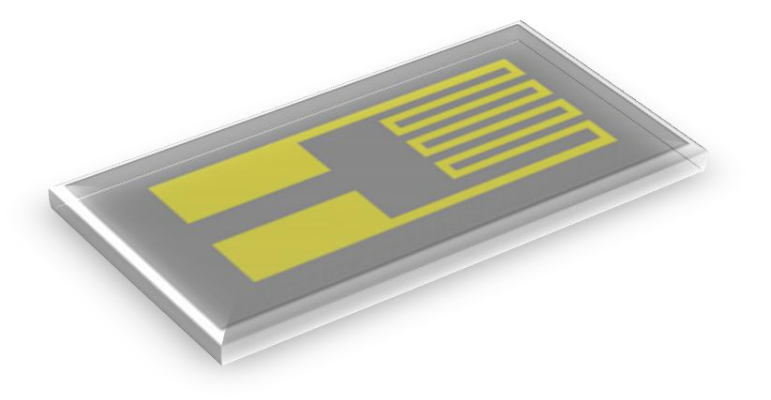
\includegraphics[height = 2.5in]{Images/serpantine.PNG}
    \caption{Illustration of serpentine thermistor. Image obtained from \cite{Sensors2018}}
    \label{fig:serpentine}
\end{figure}

Now that the geometry of the sensor was planned, the material choice was the next consideration. The material that the sensor was made of needed to produce the largest resistance change for the approximately 15\textcelsius{} temperature change. The dimensions that were decided on were based on the limitations of the fabrication methods used in the lab. This meant that the width of the serpentine wire as well as the gaps between wires was going to be $10 \mu m$. The height of the metal deposition will be $200nm$ on recommendation from professor Prakash to avoid fragility issues. Information on four of the most common metals used in thermal sensors was put together in the following tables. the calculated values are for a sensor patch $1cm^2$ in size. The results for the base resistance of each type of metal is seen in table \ref{tab:baseResistTable}.

\begin{table}[h!]
    \centering
    \caption{Resistivity of base metals}
    \label{tab:baseResistTable}
    \begin{tabular}{|c|c|c|}
        \hline
        Material & Resistivity ($\rho$)[$\Omega  m$] & $R_o$ at 20\textcelsius{} \\
        \hline
        Nichrome & $110*10^{-8}$ & $2.75M\Omega$ \\
        \hline
        Platinum & $10.6*10^{-8}$ & $265K\Omega$ \\
        \hline
        Nickel & $7*10^{-8}$ & $175K\Omega$ \\
        \hline
        Chromium & $12.5*10^{-8}$ & $312.5K\Omega$ \\
        \hline
    \end{tabular}
\end{table}

Something to note in table \ref{tab:baseResistTable} is that nichrome has the highest base resistance by an entire order of magnitude. Nichrome is a metal that is commonly use in electrically resistive circuits like toasters. In order to see if it is the best metal to use for this sensor the change in resistance for a temperature change needed to be calculated. To do this, the base values in table \ref{tab:baseResistTable} were used to calculated the change in resistance using equation \ref{eq:ThermalRes} for a temperature change of 15\textcelsius{}. the results are shown in table \ref{tab:tempcoefficienttable}.

\begin{table}[h!]
    \centering
    \caption{Temperature coefficients of chosen metals and the change in resistance over 15\textcelsius{}.}
    \label{tab:tempcoefficienttable}
    \begin{tabular}{|c|c|c|}
        \hline
        Material & Temperature coefficient ($\alpha$) & $\Delta R$ for 15\textcelsius{} \\
        \hline
        Nichrome & $1.7*10^{-4}$ & $7.15K\Omega$ \\
        \hline
        Platinum & $3.85*10^{-3}$ & $20.8K\Omega$ \\
        \hline
        Nickel & $5.9*10^{-3}$ & $20.5K\Omega$ \\
        \hline
        Chromium & $3.0*10^{-3}$ & $36.9K\Omega$ \\
        \hline
    \end{tabular}
\end{table}

Since the metric that was used for the best metal to choose was the overall change in resistance, the best metal to choose is clearly chromium. Two sizes of thermal sensor were designed, one patch would be $1cm^2$ and the other patch would be $0.5cm^2$ so that the different sizes of sensors would be compared. With the geometry and metal chosen, the details were submitted and the design of the masks for the first round of fabrication began.


\subsection{Experimental Design \& Setup}

The sensors were fabricated with the mask that was designed to specification. The sensors were received on March 5th. The thermal sensors consisted of two clusters of four sensors. In total there were four small sensors which were $0.5cm^2$ shown in figure \ref{fig:SmallRes} and four large sensors of size $1cm^2$ shown in \ref{fig:LargeRes}. Something to keep in mind for this report is that although the sensors were labeled and kept track of individually, the large sensors and small sensors will be compared as a group.

\begin{figure}[h!]
    \centering
    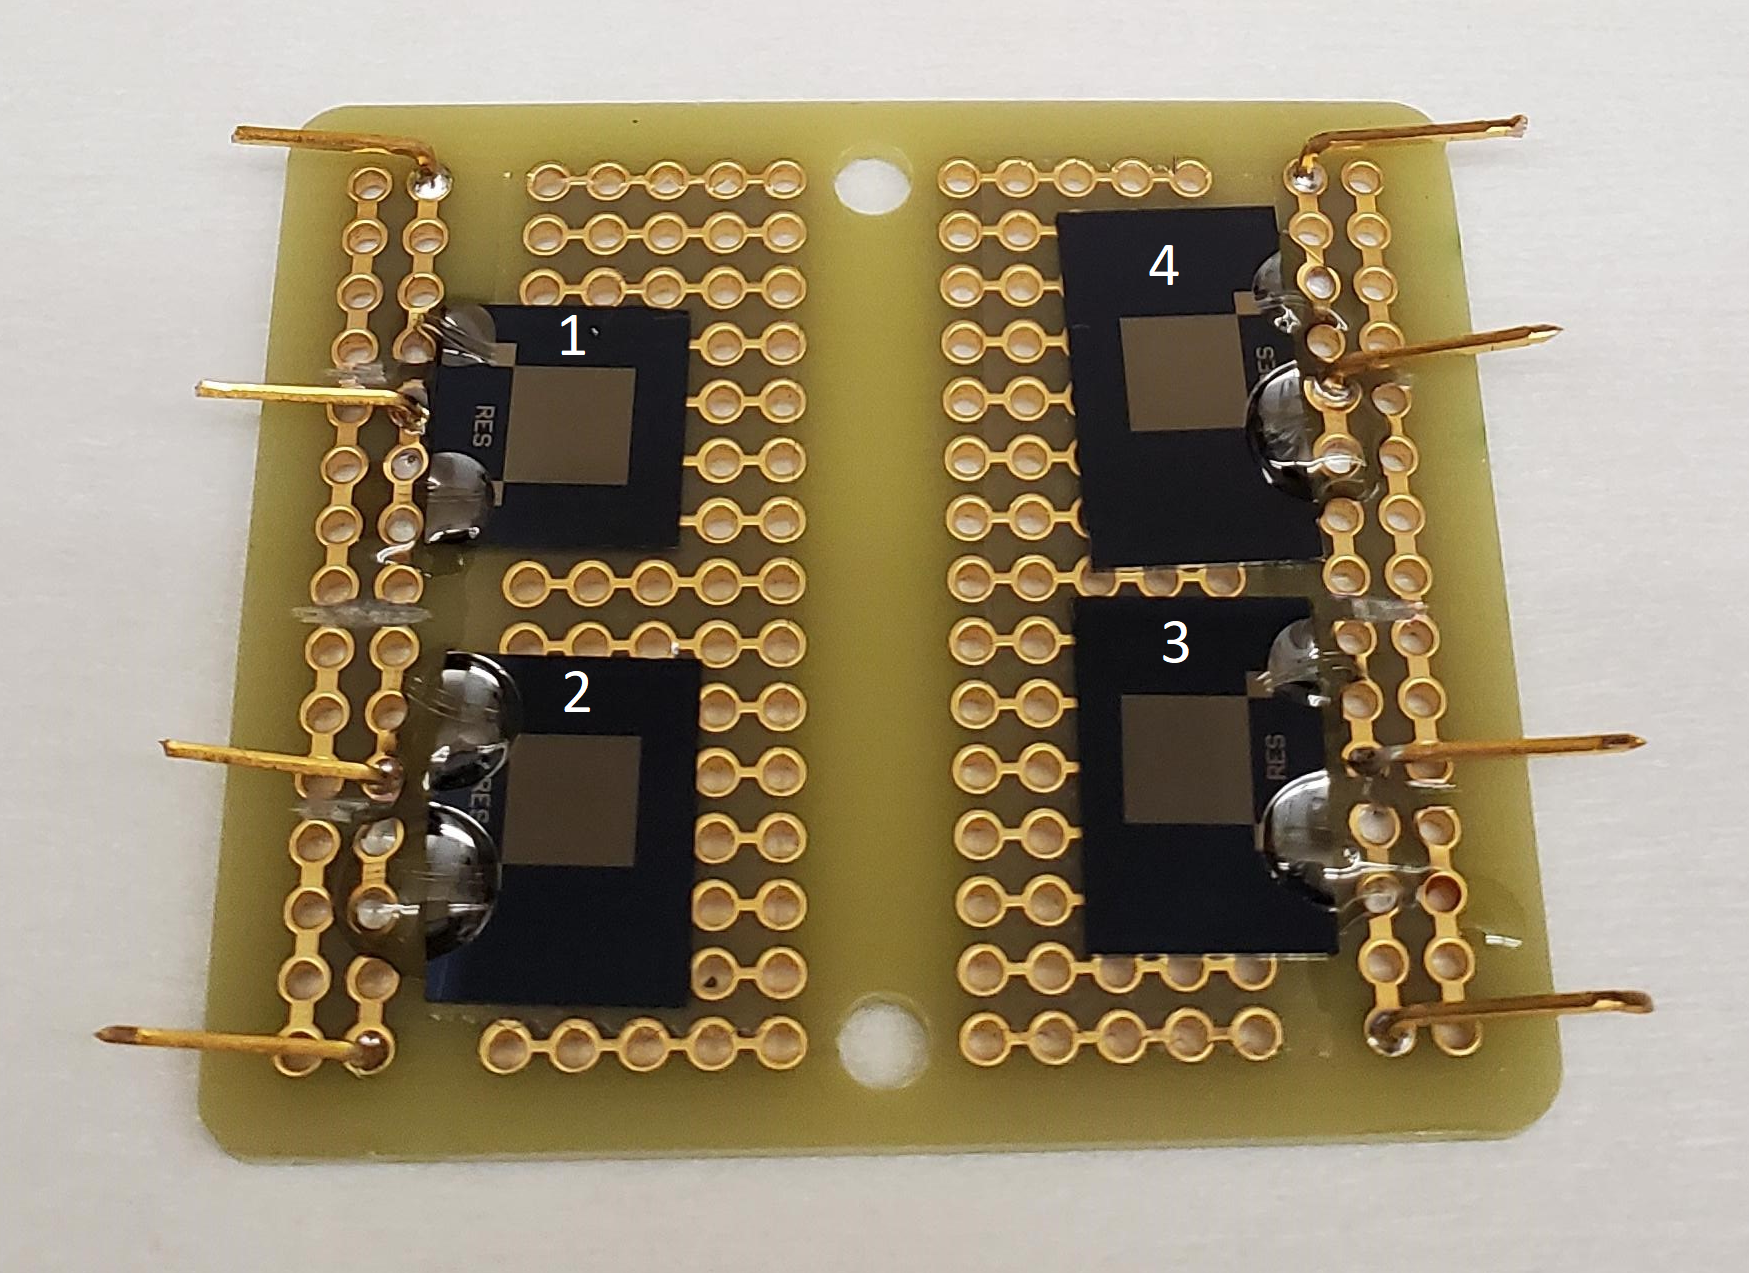
\includegraphics[height = 2.5in]{Images/SMALLRES.png}
    \caption{Fabricated small sensors attached to the breadboard.}
    \label{fig:SmallRes}
\end{figure}

The Lab technicians were kind enough to wire bond gold wires to the contact pads on the sensors and fix them to the protoboard as shown in the figures of the sensors. Something to note for later discussion is the size of the silicon chip on which the small sensors are resting, compared to the size of the silicon chip for the large sensors. The protoboards are the same size so they can be used for reference to get a feel for the relative size of the sensors. The first thing that was done with the sensors was solder extra wire to the wire contacts on the board that were put there by the lab technicians.



\begin{figure}[h!]
    \centering
    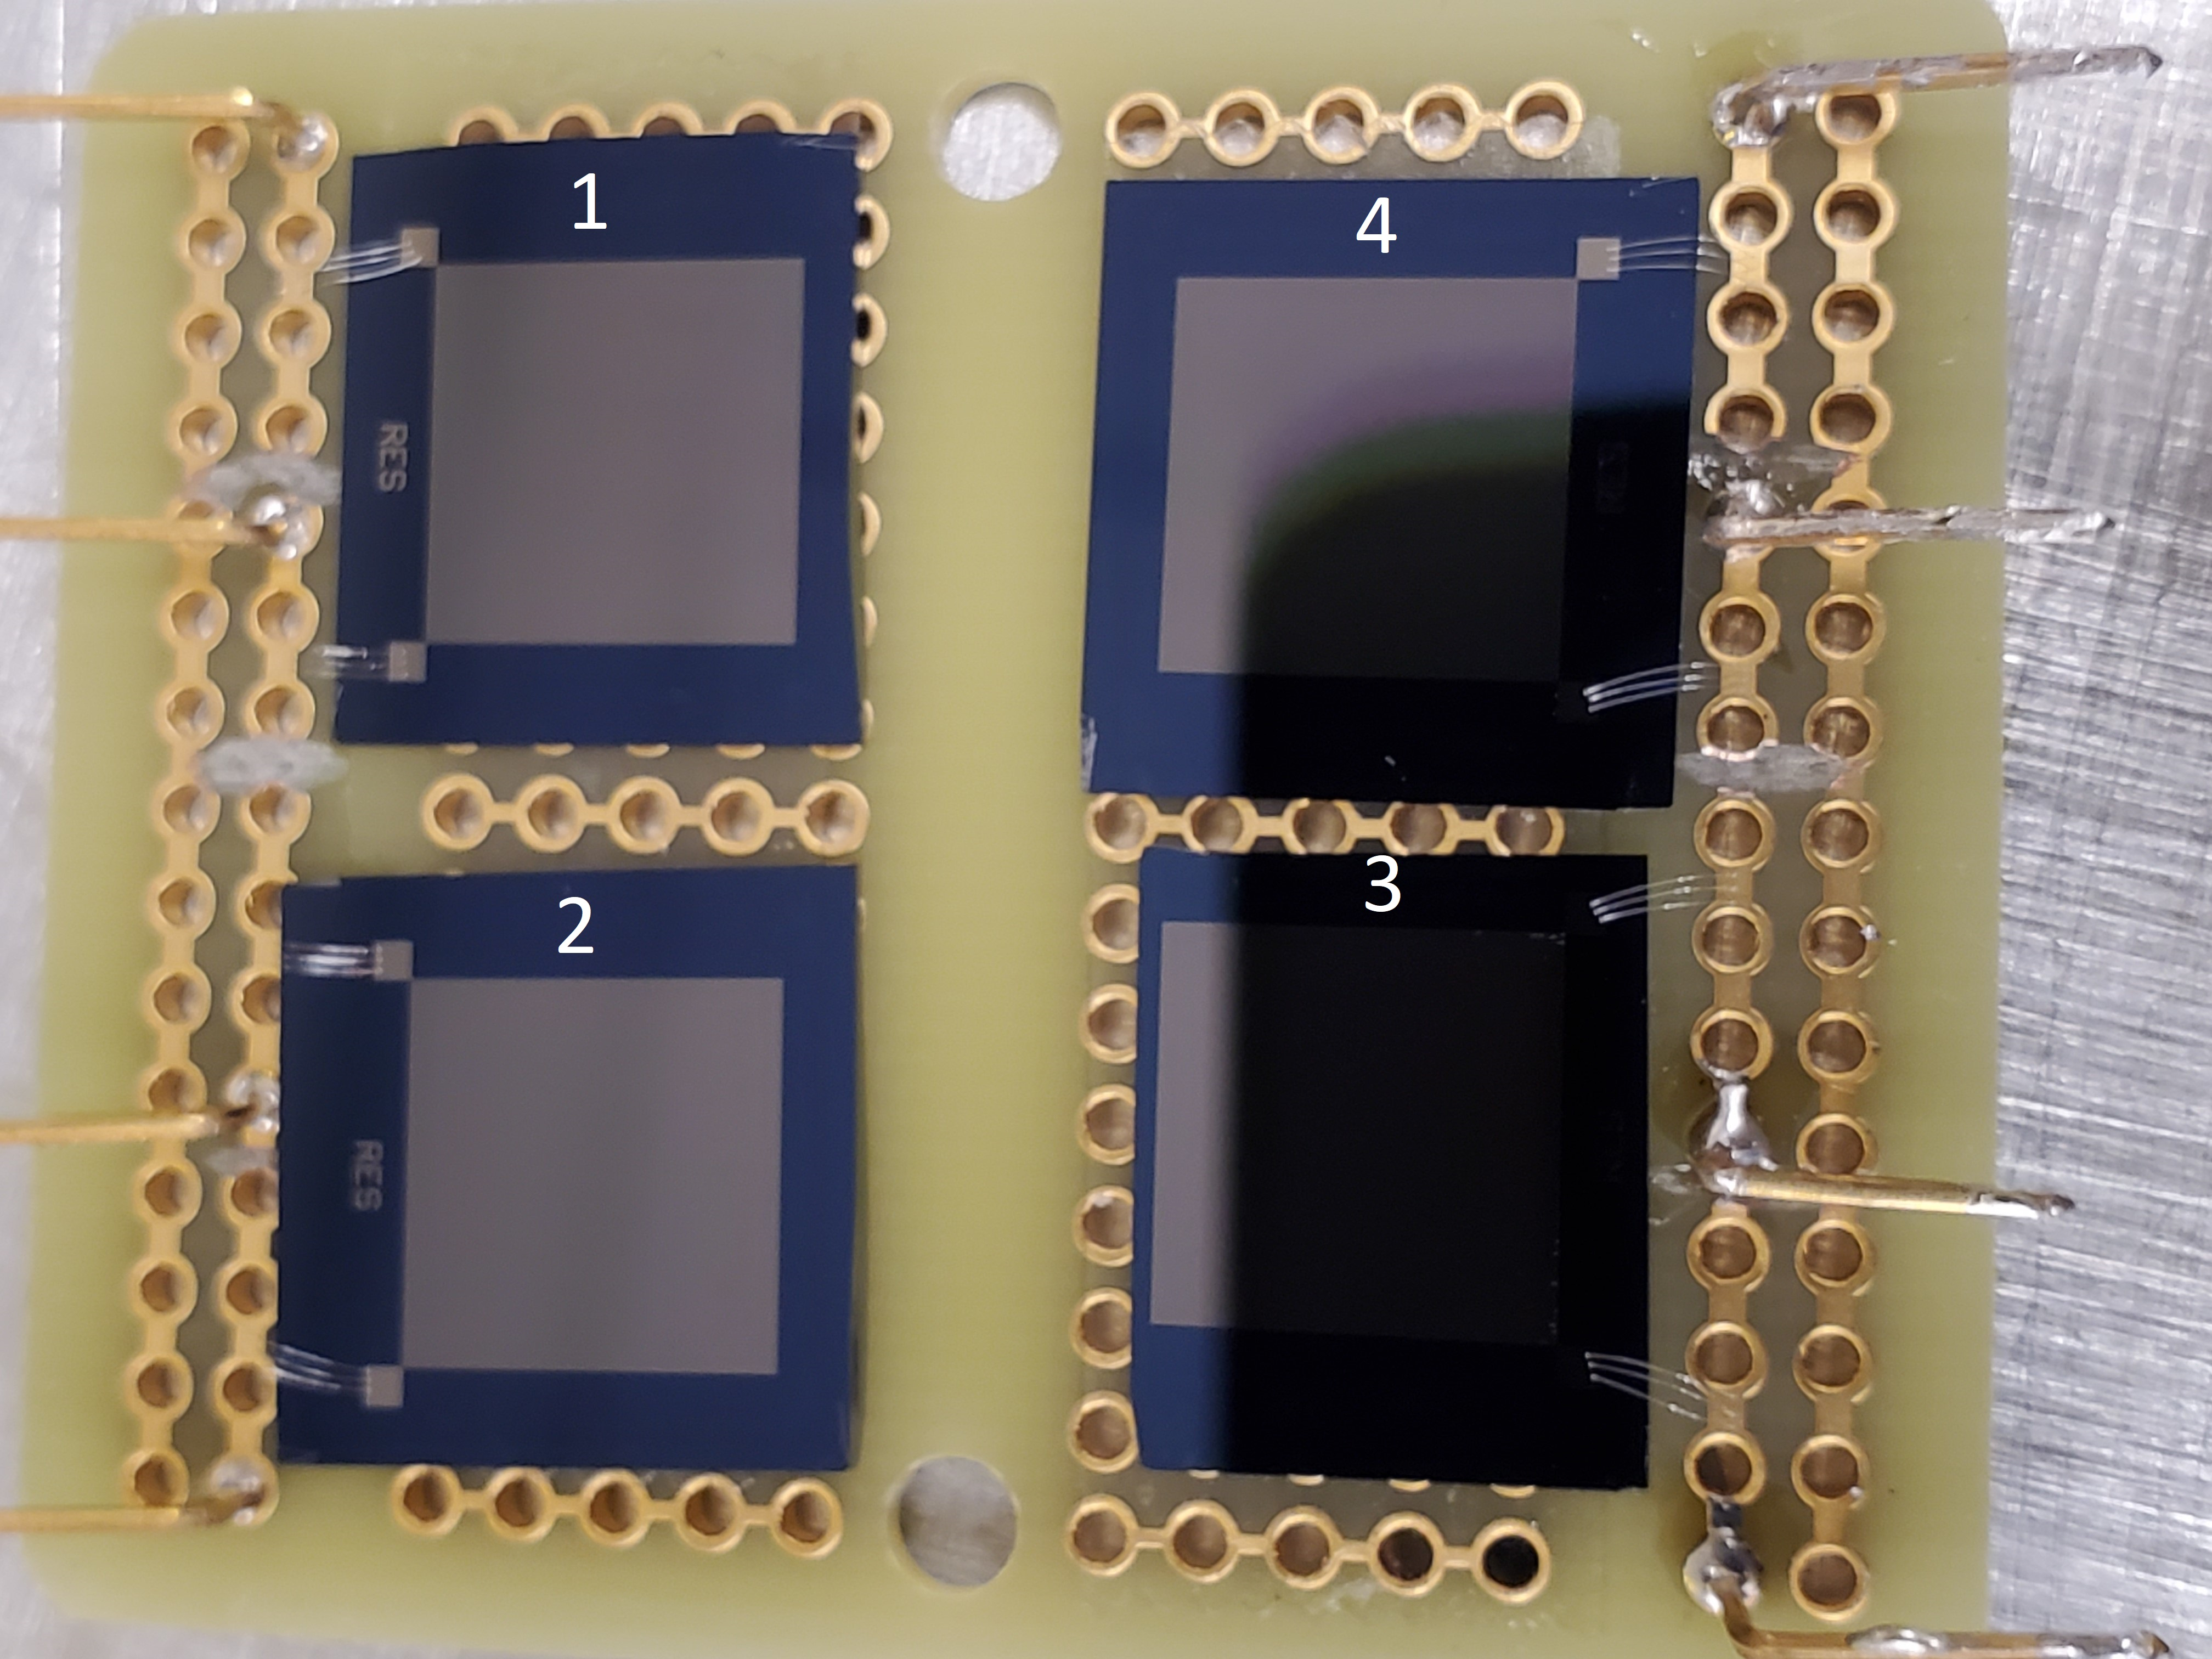
\includegraphics[height = 2.5in]{Images/LargeRes.jpg}
    \caption{Fabricated large sensors attached to the breadboard.}
    \label{fig:LargeRes}
\end{figure}

The base resistance values of the sensors were then measured and a hairdryer was used to heat them and observe a resistance change when they experienced a temperature change. This is shown in table \ref{tab:baseResistTable}. Something interesting is that no matter which sensor was tested, they all showed the same variation in resistance of $3k\Omega$. This reading was done with the digital multimeter and the hairdryer on low power. As we will see later in this report, this means that the temperature change was at least 17\textcelsius{}. There was a resistance change, so testing proceeded as planned.

\begin{table}[h!]
    \centering
    \caption{Resistance values and change in resistance when heat was applied}
    \label{tab:BaseResistTable}
    \begin{tabular}{|c|c|c|c|}
        \hline
        & Sensors & $R_o$ & $\Delta R$  \\
        \hline
        \multirow{4}{*}{Small fig(\ref{fig:SmallRes})} & 1 & $410k\Omega$ & $3k\Omega$ \\
        & 2 & $406k\Omega$ & $3k\Omega$  \\
        & 3 & $445k\Omega$ & $3k\Omega$  \\
        & 4 & $375k\Omega$ & $3k\Omega$  \\
        \hline
        \multirow{4}{*}{Large fig(\ref{fig:LargeRes})}& 1 & $1.54M\Omega$ & $3k\Omega$  \\
        & 2 & $1.76M\Omega$ & $3k\Omega$  \\
        & 3 & $1.66M\Omega$ & $3k\Omega$ \\
        & 4 & $1.54M\Omega$ & $3k\Omega$  \\
        \hline
    \end{tabular}
\end{table}

The Adafruit FLORA was the micro controller that was chosen for this project. It has 4 10-bit analog to digital inputs which gave us 1024 values of sensor signal resolution. For initial testing, the FLORA was attached to the computer and read values from one of its analog inputs. This reading was then printed to the serial port and captured with CoolTerm, which would copy the serial port data and write it to a .txt file. The data was collected and then was processed in MATLAB after collection had finished. 
\par
The entire testing setup is shown in figure \ref{fig:Testing Setup}. This is the home laboratory that was used. On the right side of the image shows the hairdryer used for applying heat to the sensors, below the hairdryer is the sensor cluster with the sensor being tested which was resting on top of the calibration thermometer. This thermometer was a cheap outdoor thermometer that was picked up from home hardware for less than \$10. The reason this thermometer was chosen was because the back of the thermometer has an opening that exposes the bulb. When testing each sensor, the bulb of the thermometer was as close to the sensor being tested as possible. 

\begin{figure}[h!]
    \centering
    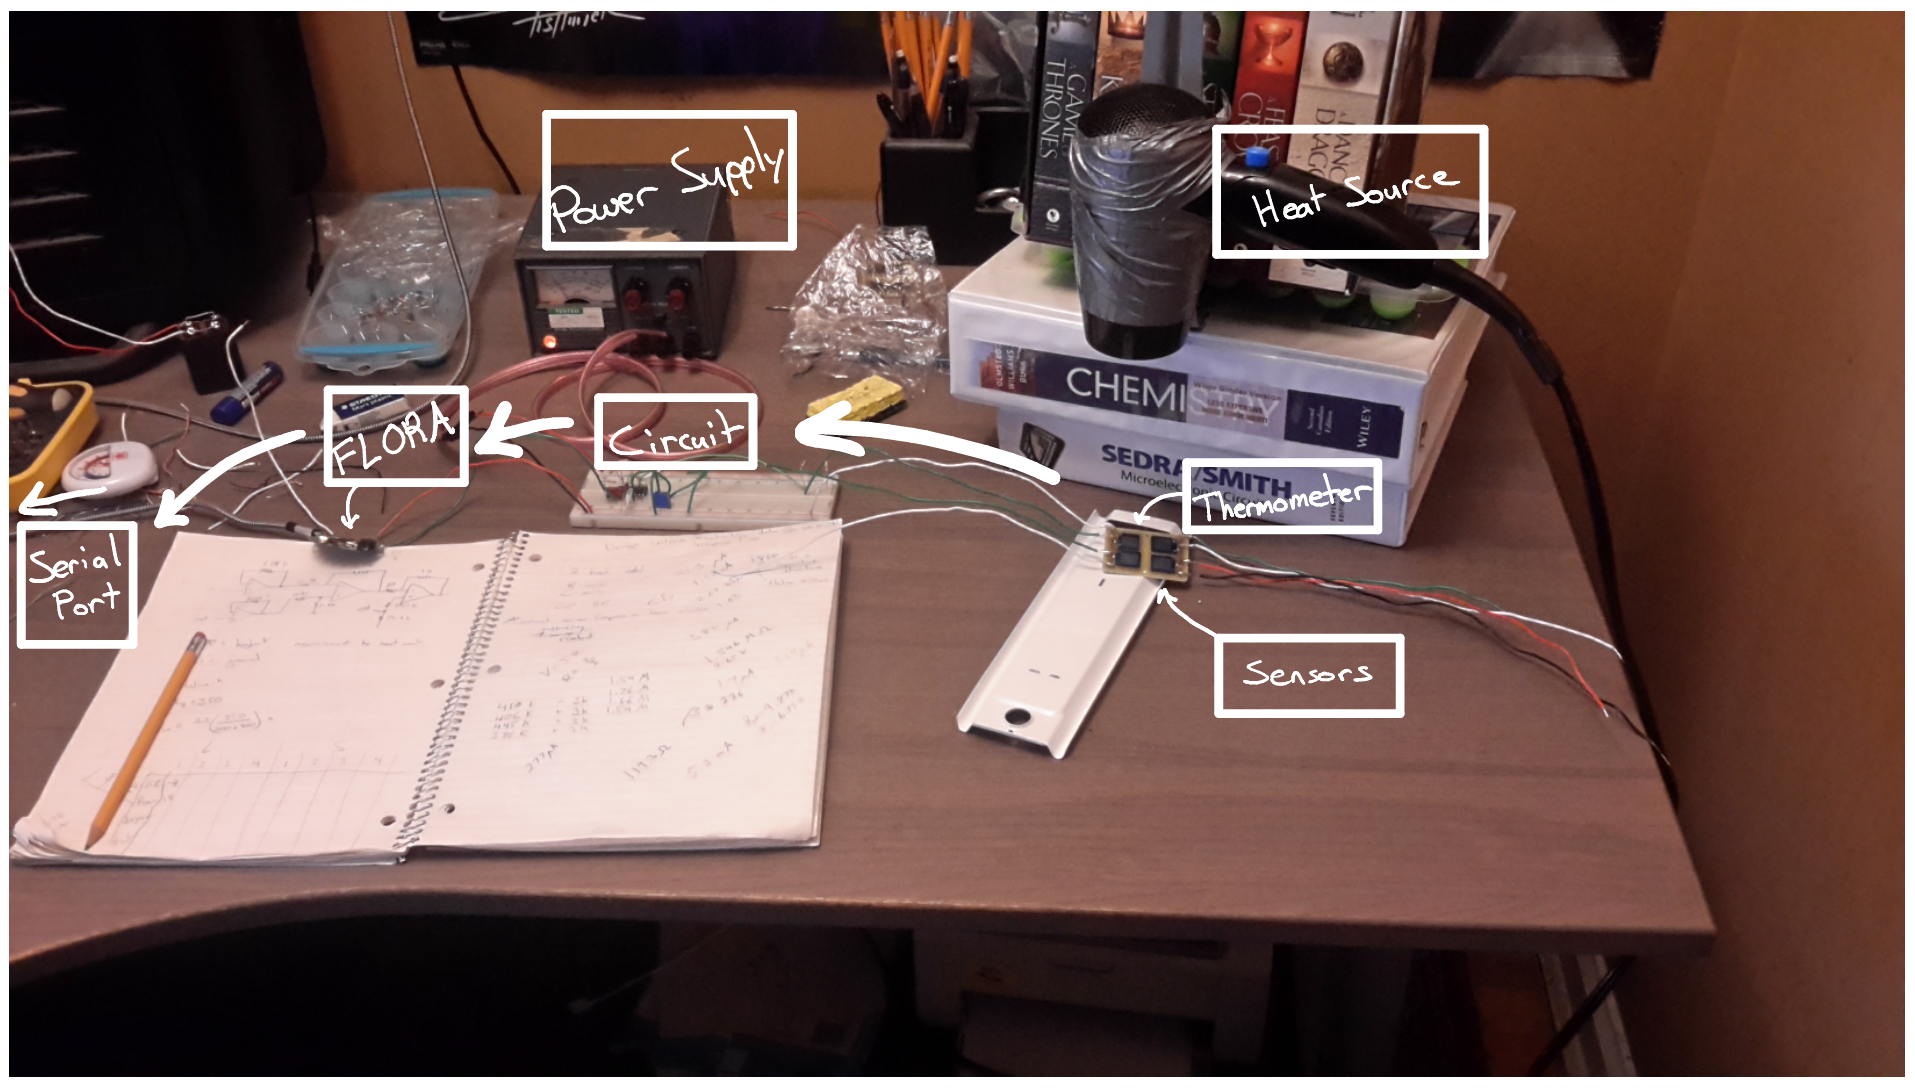
\includegraphics[height = 3in]{Images/TestingSetup.png}
    \caption{Testing Environment with annotations of components}
    \label{fig:Testing Setup}
\end{figure}

Left of that is the processing and conditioning circuit that would produce a DC signal from 0 to 3.3V for a calculated temperature range of 0 to 50\textcelsius{}. The initial circuit used to test the signal is shown in figure \ref{fig:InitialCuircuit} and will be discussed in a shortly. To the left of the circuit is the FLORA micro controller which took the circuit signal as input and printed a 10 bit analog to digital signal to the serial port as output. As previously mentioned, the serial port signal would then be processed.\par

In order to read the small change in resistance as a signal, it needed to be amplified. This amplification was done through a differential amplifier as seen in figure \ref{fig:InitialCuircuit}. The RTD thermal sensor was connected in a voltage divider setup with a top resistor of approximately equal value to the resistor. This made the voltage across the RTD half of the input voltage and also maximized the swing of the voltage due to changes in resistance of the RTD. This input voltage was sent though a buffer as to not impact the sensitive differential amplifier. A reference voltage also needed to be created to use the differential amplifier most effectively. The reference voltage was created with a $50k\Omega$ potentiometer. For each sensor that was being testing, the potentiometer was adjusted such that the signal at room temperature gave the lowest stable reading in the serial output, which was approximately 100 out of the potential 1024 values from the 10 bit input. This made sure that there was plenty of room to increase the signal.

\begin{figure}[h!]
    \centering
    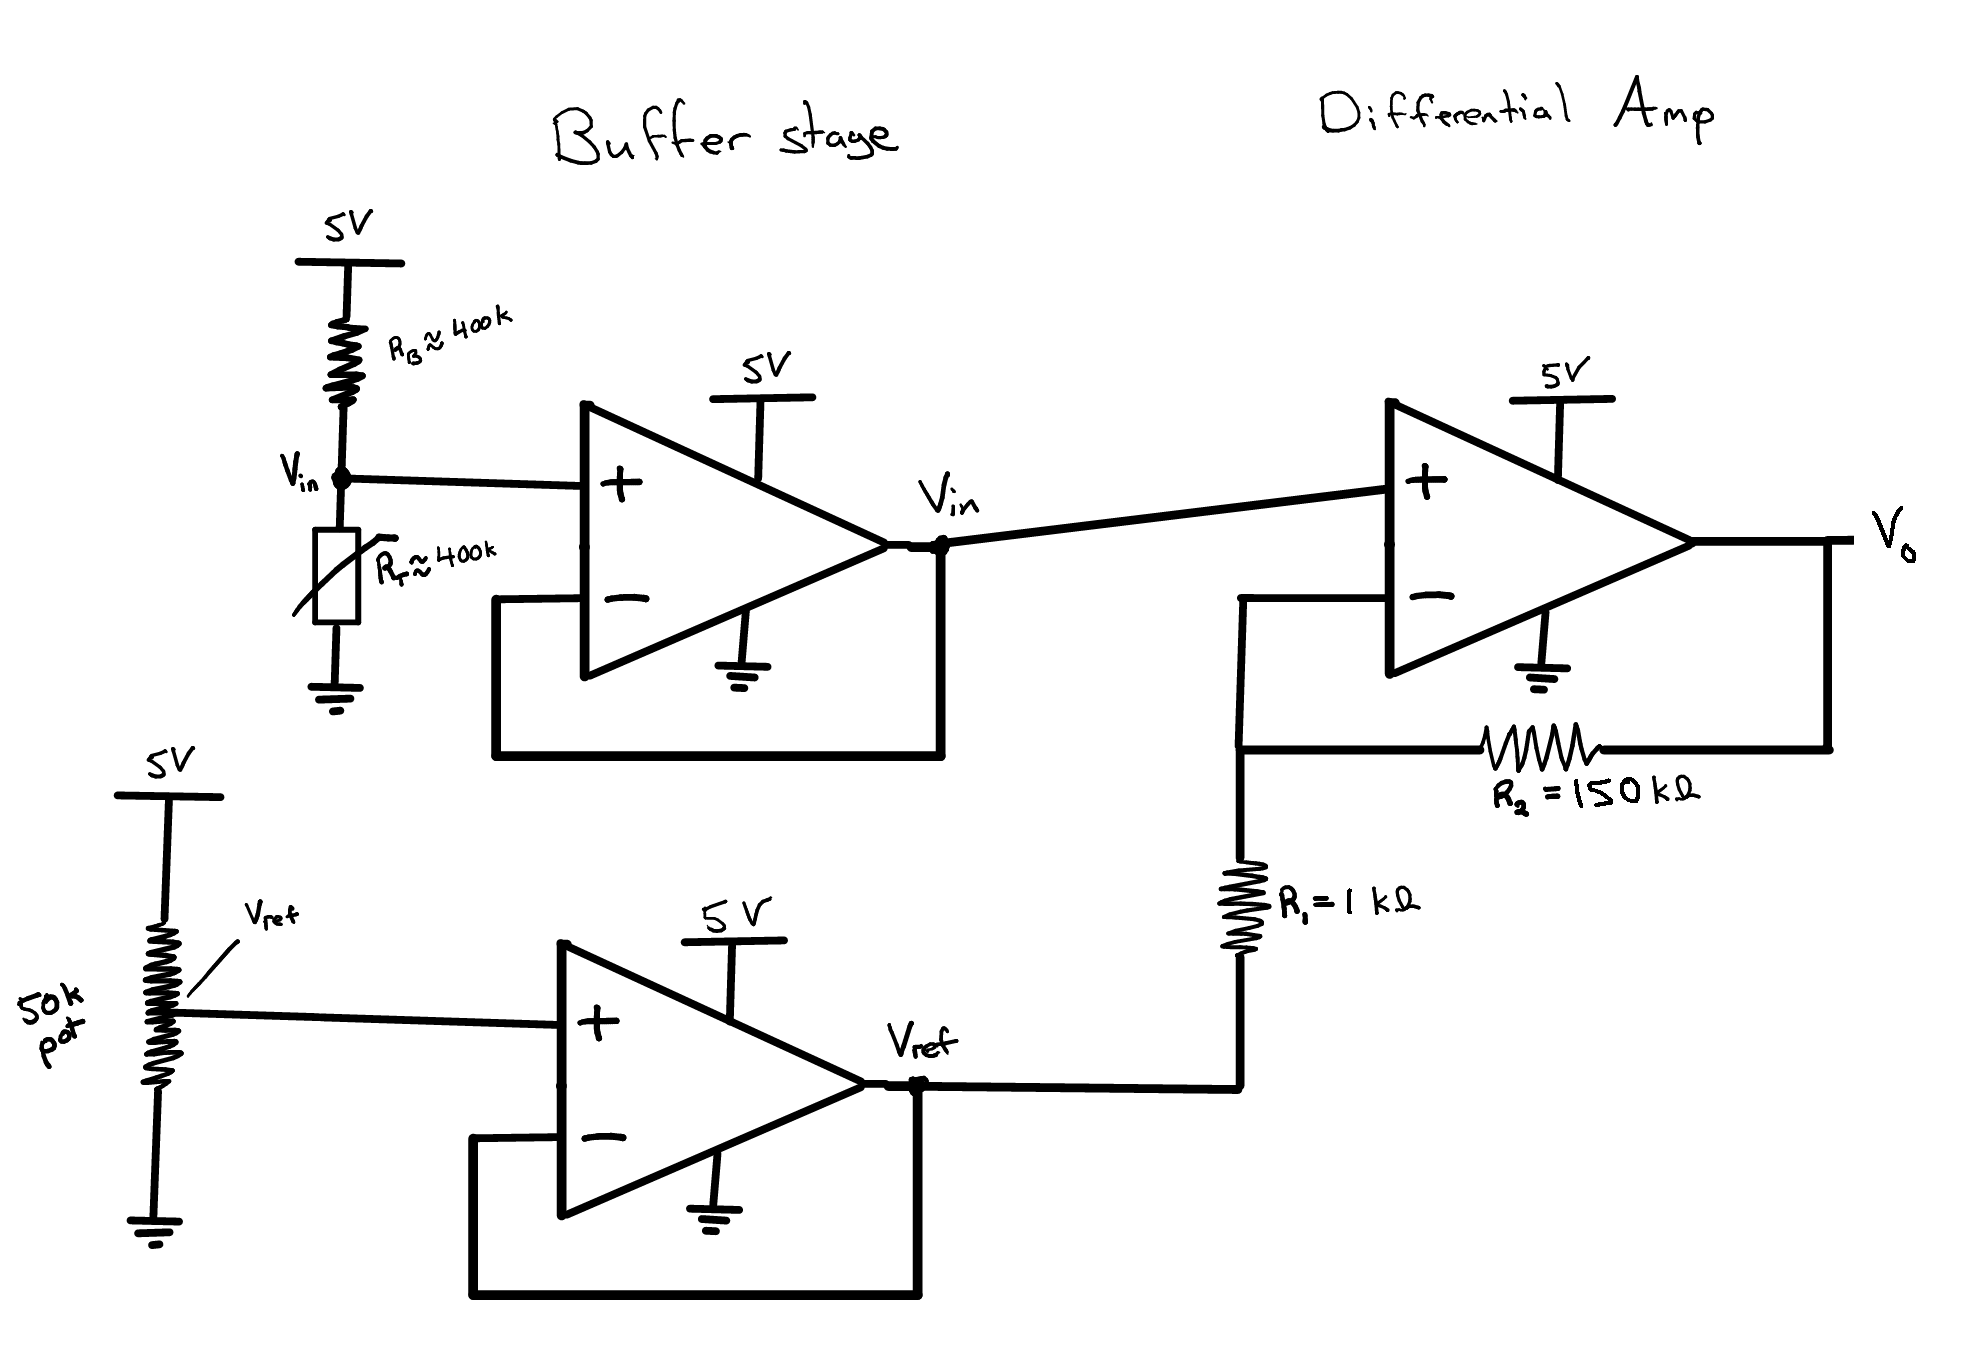
\includegraphics[height = 2.5in]{Images/initial_circuit.png}
    \caption{Initial circuit used to read data from the sensor.}
    \label{fig:InitialCuircuit}
\end{figure}

The amplification was done in a non inverting fashion. since the reference voltage was also sent through a buffer, all that needed to be done was to calculate what gain was necessary to turn the small voltage increase into the 3.3V maximum. The measured values of Voltage for room temperature and hairdryer temperature for small sensor 1 are shown in table \ref{tab:DiffAmpParams}, as well as the target output voltage minimum and maximum.

\begin{table}[h!]
    \centering
    \caption{Voltage parameters for differential amplifier}
    \label{tab:DiffAmpParams}
    \begin{tabular}{|c|c|c|c|}
        \hline
        $V_{i_{min}}$ & $V_{i_{max}}$ & $V_{o_{min}}$ & $V_{o_{max}}$\\
        \hline
        2.44 & 2.46 & 0.05 & 3.3 \\
        \hline
    \end{tabular}
\end{table}

The voltage swing from the temperature change produces a small signal of $20mV$. In order to calculate necessary gain for the non inverting amplifier the equation below was used:

\begin{equation}\label{eq:GainS}
    A = \frac{V_{o_{max}}-V_{o_{min}}}{V_{i_{max}}-V_{i_{min}}} = \frac{3.25V}{0.02V} = 162.5 V/V
\end{equation}

 A gain factor of 162.5 would have been ideal. But the resistors that were available in the home lab were all in a plastic bag full of old, used resistors. Figure \ref{fig:Testing Setup} shows some of the resistors that had been pre-organized in an ice tray to the left of the power supply. It would suffice to say that the required resistors were not easily available, so values were selected to give a gain as close as possible to the value calculated in equation \ref{eq:GainS}. This ended up being a non inverting combination of $1k\Omega$ and $150k\Omega$ resistors, creating a gain of approximately 150.\par
 
 The output of this sensor was fed into the FLORA and there was some success in the voltage increase over time when a hairdryer was blowing on the circuit, as seen in figure \ref{fig:UnfilteredFLORA}. 

\begin{figure}[h!]
    \centering
    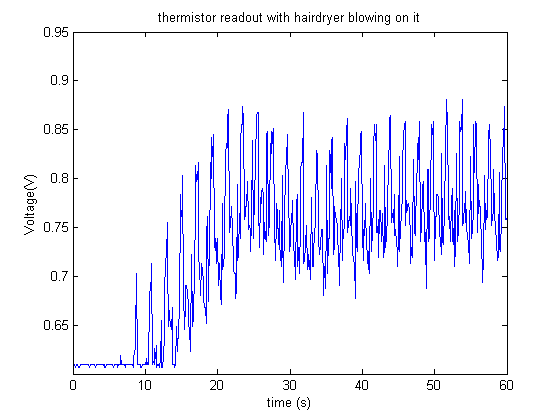
\includegraphics[height = 2.5in]{Images/UnfilteredOutput.png}
    \caption{Unfiltered data captured when a hairdryer is blowing on it.}
    \label{fig:UnfilteredFLORA}
\end{figure}

When the signal was observed from the oscilloscope the high frequency components were clearly visible. figure \ref{fig:UnfilteredOutput} shows the output of the oscilloscope

\begin{figure}[h!]
    \centering
    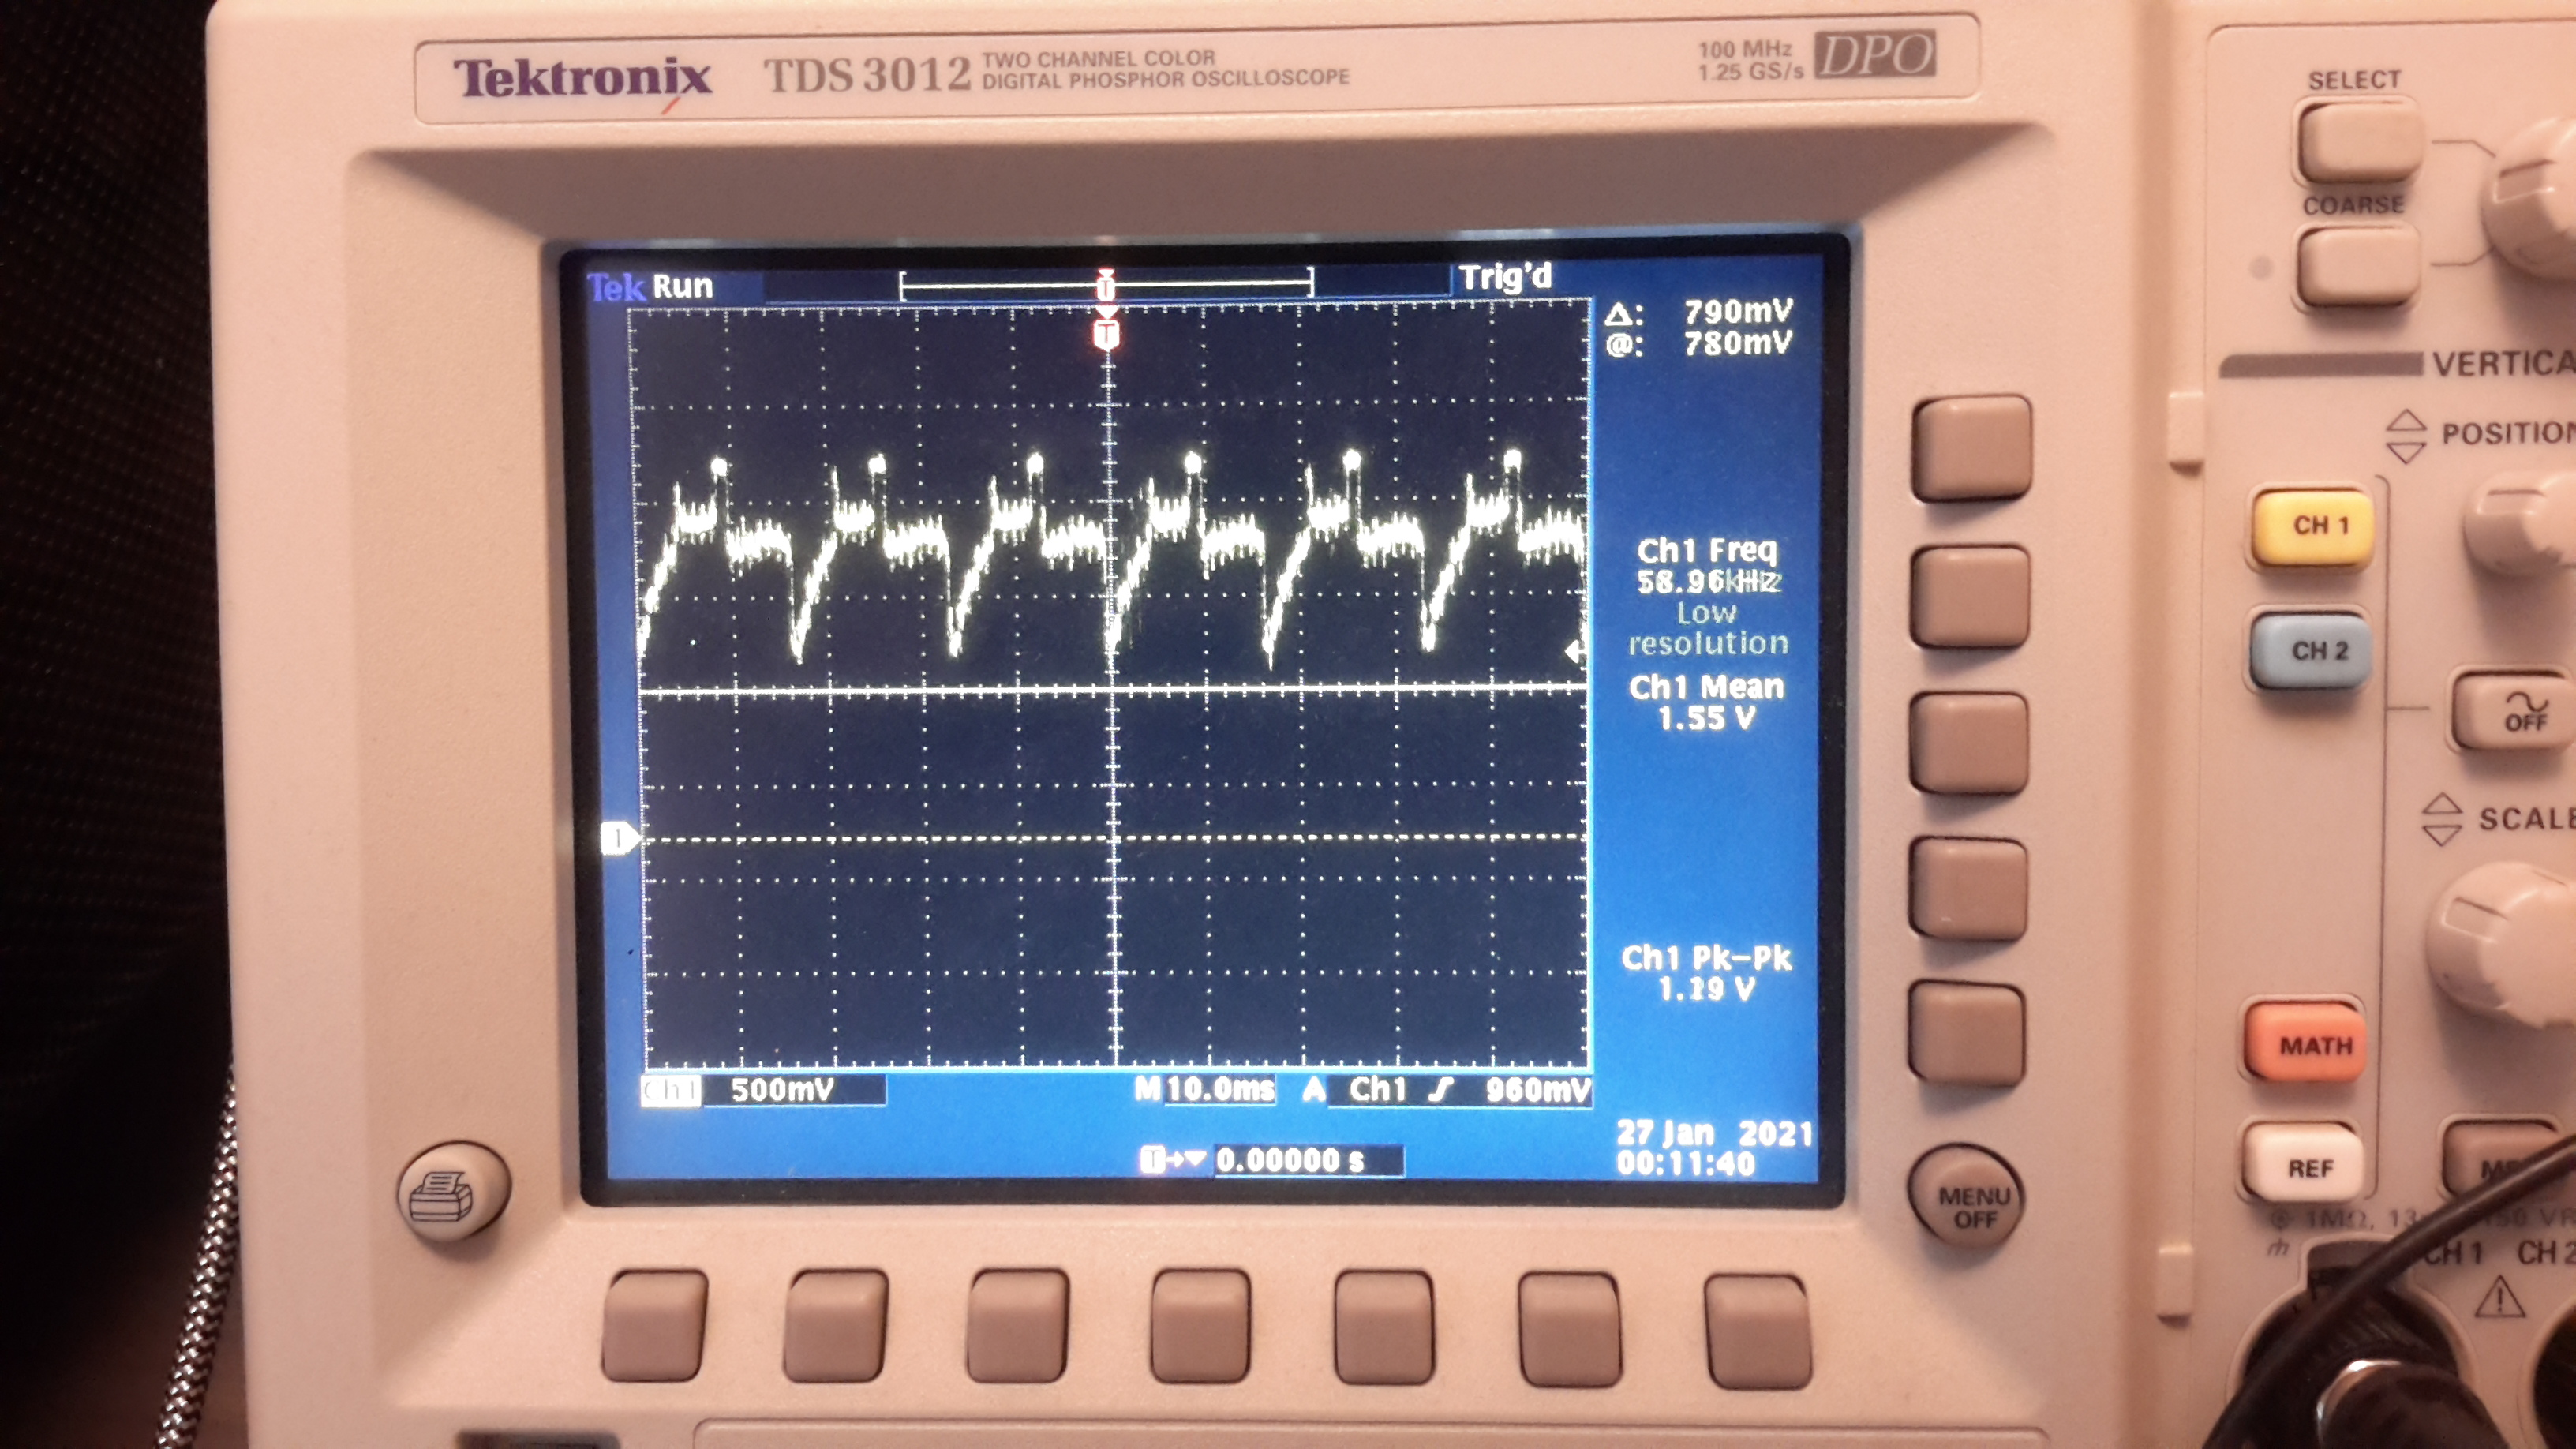
\includegraphics[height = 2.5in]{Images/TempSensOutUnfiltered.jpg}
    \caption{Unfiltered output of the sensor, including high frequency components.}
    \label{fig:UnfilteredOutput}
\end{figure}


It was clear that the high frequency components needed to be filtered out of the signal with a low pass filter. Figure \ref{fig:ConditioningCircuit} shows the final circuit that was created with the low pass filter cleaning the output of the differential amplifier. This low pass circuit has two 'RC' filters that both have cutoff frequencies below 10Hz. The goal was to get the cuttoff frequency as low as possible with the components on hand since the only signal of interest was the DC signal. 




\begin{figure}[h!]
    \centering
    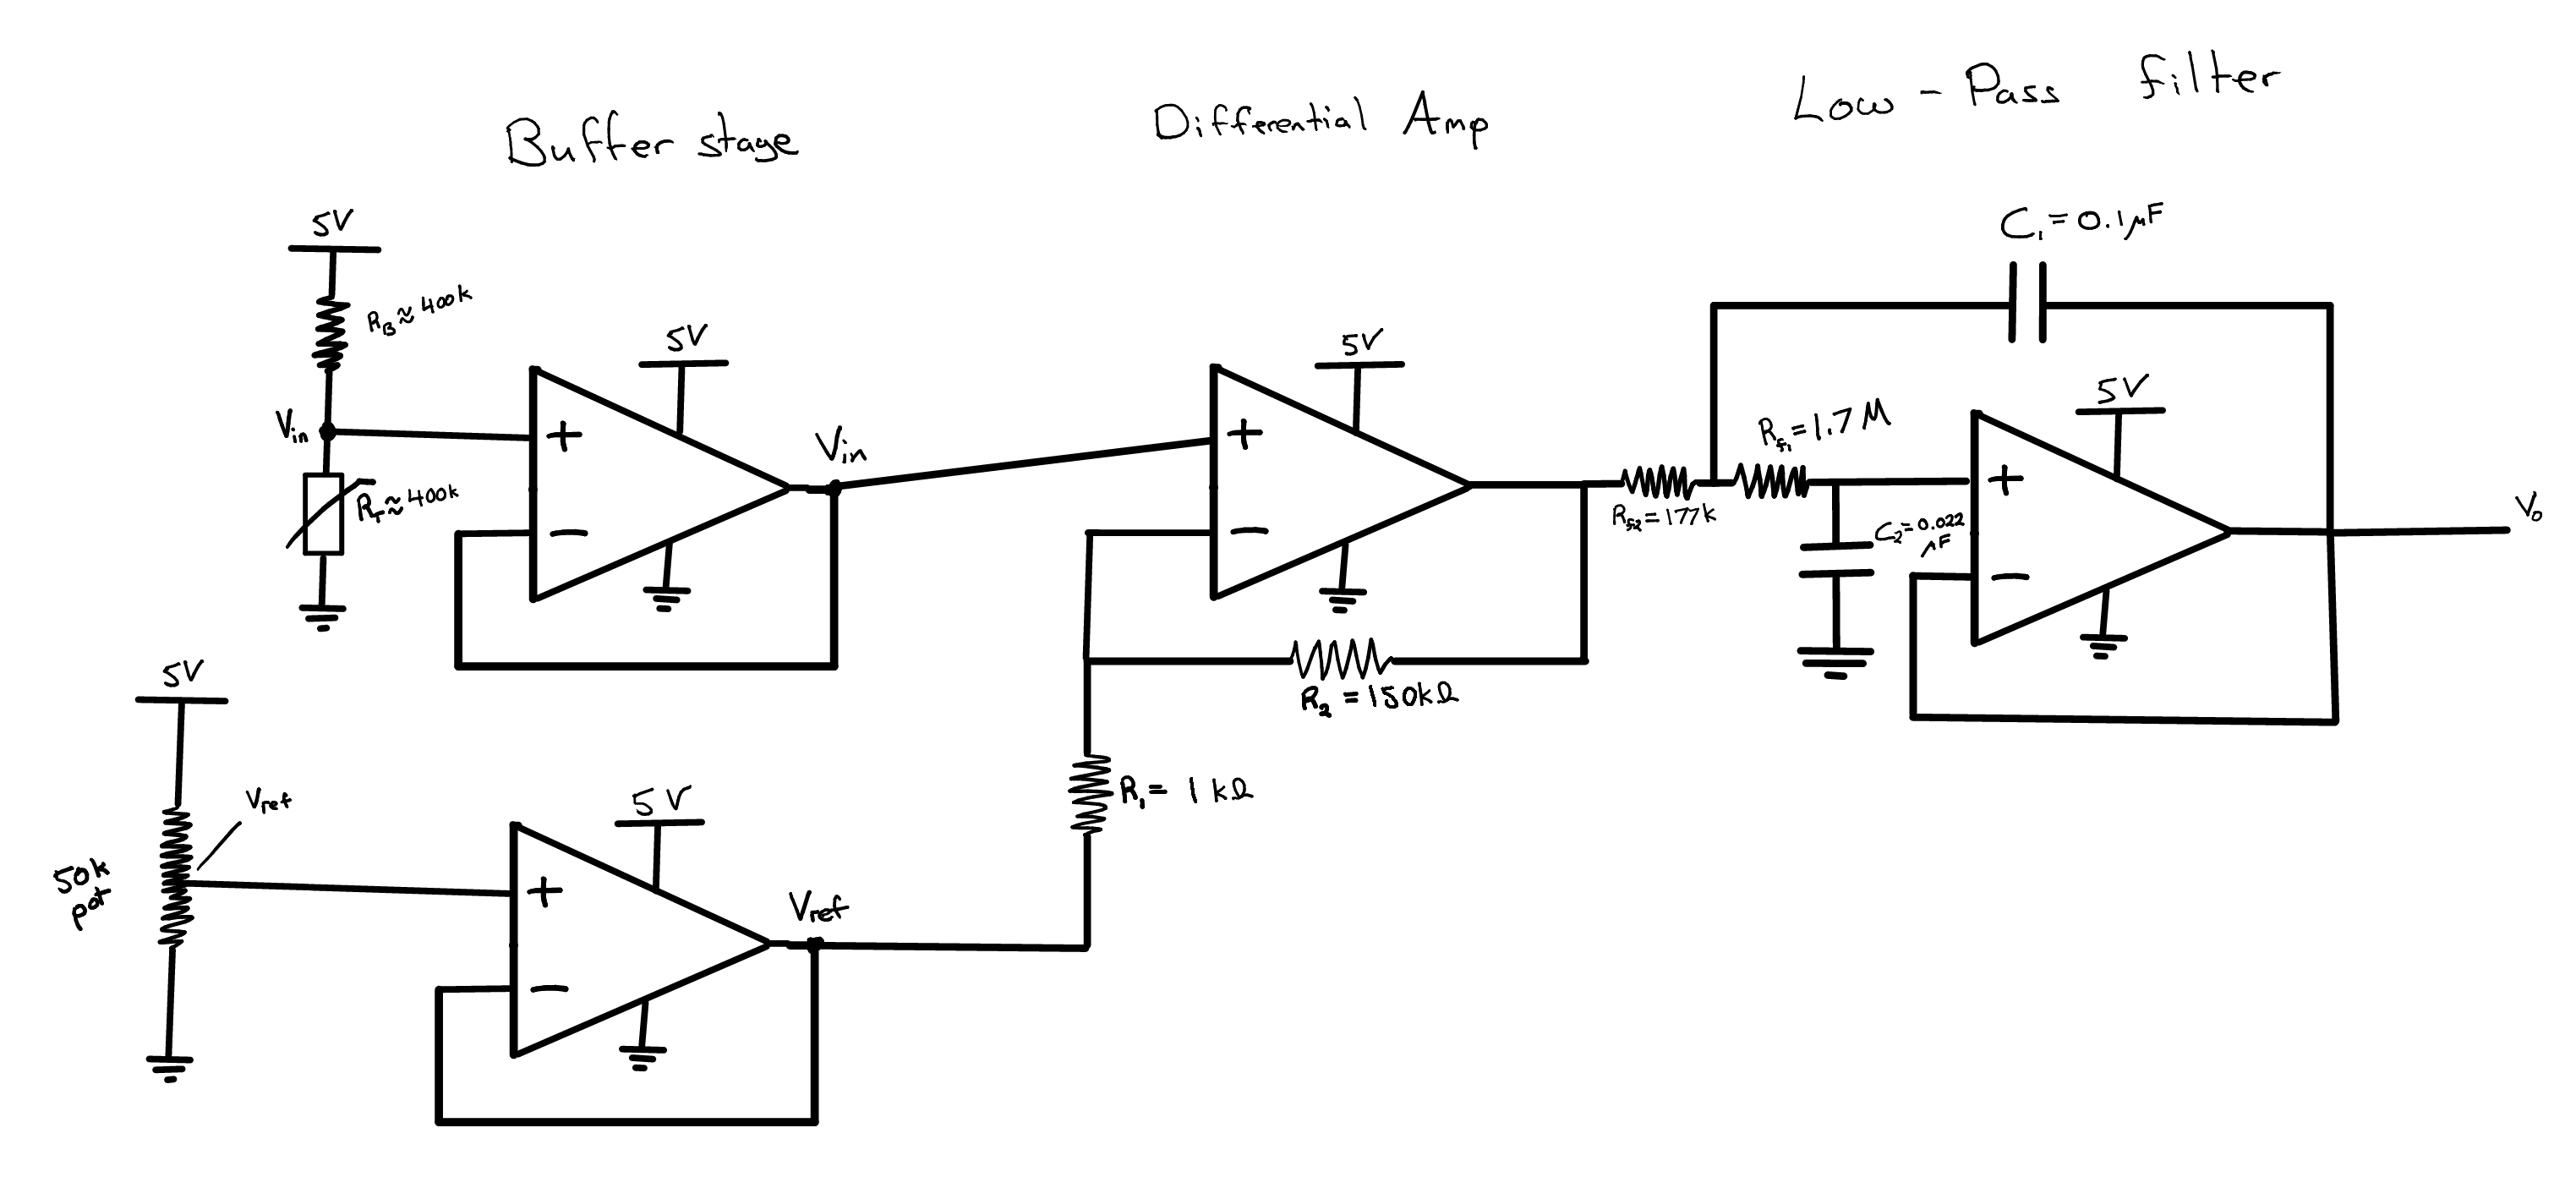
\includegraphics[height = 2.5in]{Images/ThermistorFilter.png}
    \caption{Conditioned circuit used to filter out the high frequency noise.}
    \label{fig:ConditioningCircuit}
\end{figure}

Once the filter was in place, the output signal from the conditioning circuit was smoothed out, as seen in figure \ref{fig:FilteredOutput}. 


\begin{figure}[h!]
    \centering
    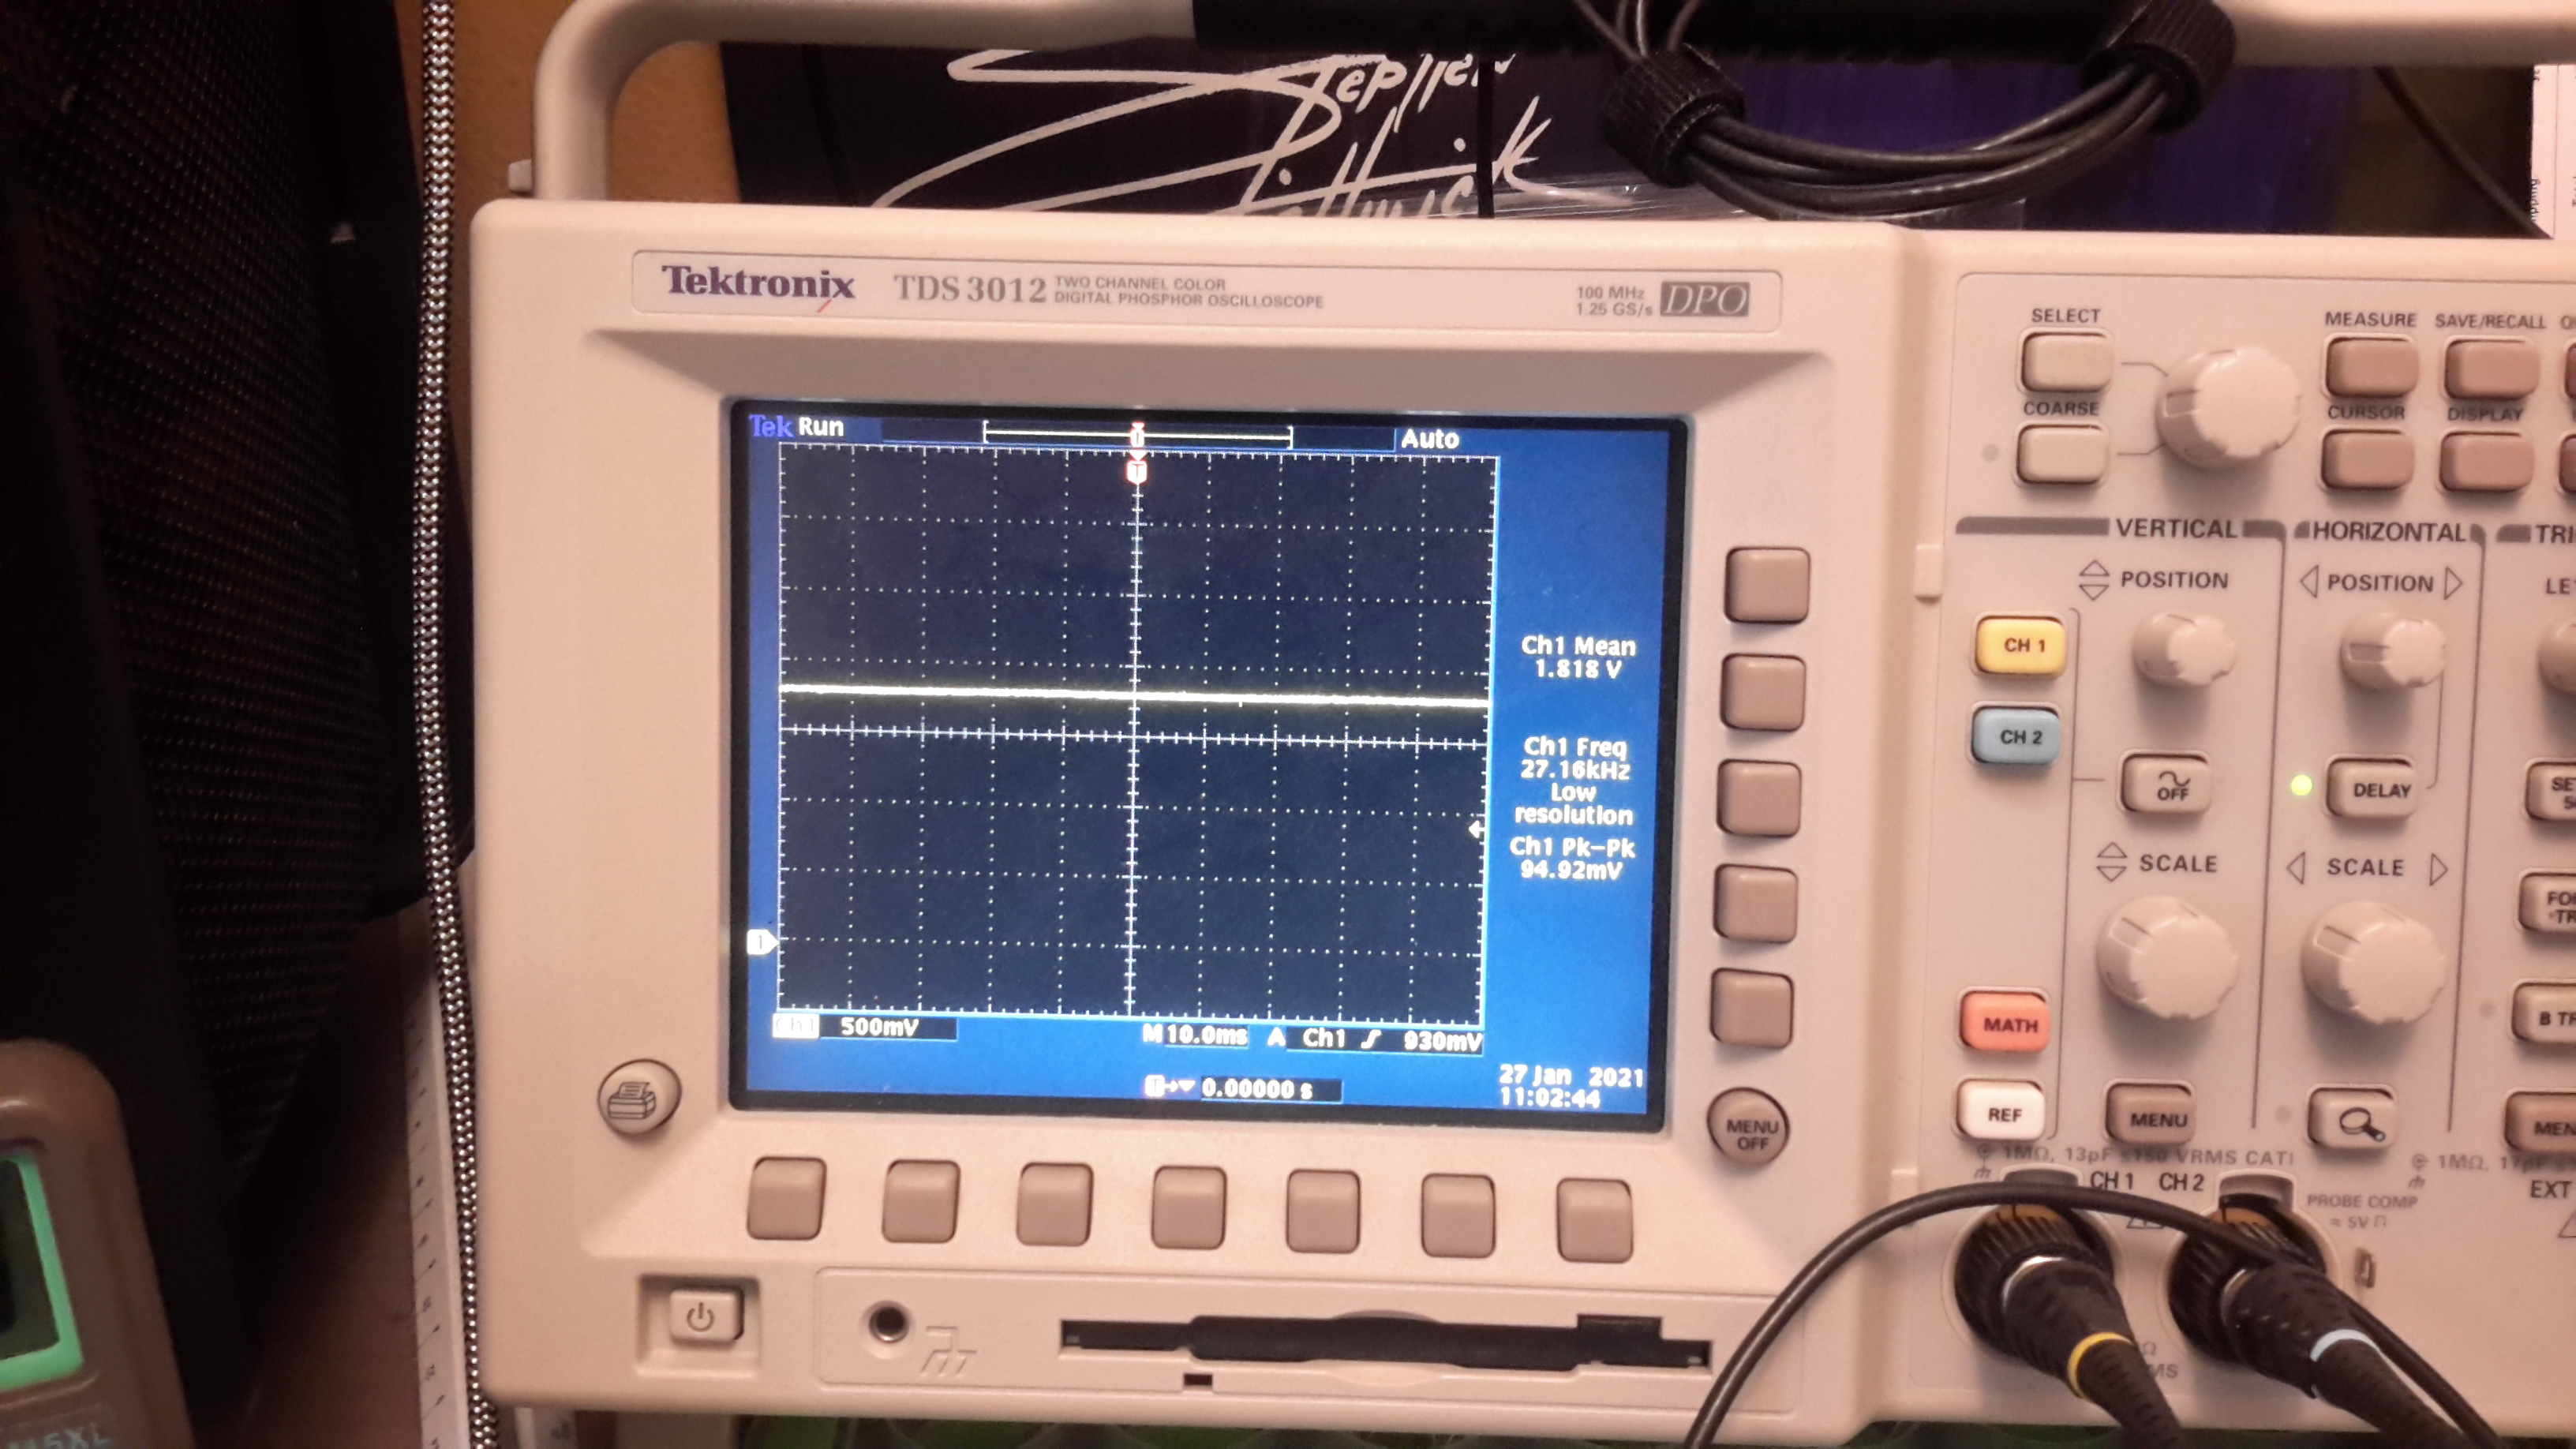
\includegraphics[height = 2.5in]{Images/TempSensOutFiltered.jpg}
    \caption{Filtered output of the sensor. With frequency noise filtered out.}
    \label{fig:FilteredOutput}
\end{figure}

 Now that the signal could be read into the FLORA and collected with some degree of accuracy. Preliminary testing could begin.






\subsection{Evaluation \& Measurement Technique}

Each sensor was calibrated according to its own response to the calibration measurements. Although there was only two sources of constant temperature to use as calibration, the temperature response of the sensors should have been linear in nature so having two points would produce sensors with a reasonable degree of accuracy. The calibration points was room temperature, which at the time of testing was approximately 12\textcelsius{}, and hair dryer temperature which ranged from 30\textcelsius{} to 33\textcelsius{} depending on how long it had been previously running.\par

Data collection happened over the course of 5 minutes and a histogram was collected to produce a mean and standard deviation for precision and accuracy metrics. This was done for both calibration points and then the calibration values were hard coded into the Adafruit FLORA and temperature readings were taking of both the wrist and the underarm to get multiple readings on the body.



\subsection{Hardware \& Software Tools}
    \subsubsection{Selection of appropriate tools and justification}
    
    The tools needed for this project were;
    
    \renewcommand{\theenumi}{\arabic{enumi}}
    \begin{enumerate}
        \item Adafruit FLORA
        \item CoolTerm
        \item MATLAB
        \item Digital Multimeter (DMM)
        \item Thermometer
    \end{enumerate}
    
    The primary decision that needed to be made about this project early on was to decide on the microcontroller for the readout and processing system. It was originally planned to create our own surface mount flexible circuit boards on Kapton and then mount a stand alone microprocessor on it, but due too time constraints, we opted for the prefabricated FLORA board instead. The reason this board was chosen was because it was recommended by Nagui Mikhail. 
        
    CoolTerm is a piece of software that I found that copied the signal from a COM port and replicated it and gave the option of storing the values into a .txt file. This capability was crucial because although the Arduino IDE would display values from the serial port, there was no way to access them. I had begun looking into writing my own C++ code to accomplish this when i found CoolTerm in Roger Meier's website\cite{CoolTerm}.\par
        
    The last piece of software necessary for this project was MATLAB. This was my first programming language that I actually enjoyed so I knew it well and could do a lot of numerical analysis. However my version was out of date and I didn't have access to the histogram function which came out in 2018. So it required an update.\par
    
    The digital multimeter was supplied by the school and was used with 10mV precision.
       
    The thermometer was just some cheap way of reading the atmospheric temperature near the sensor. I did shop around for better thermometers however the more accurate thermometers with exposed bulbs were candy thermometers and they have a minimum temperature of 25\textcelsius{}.\par
    
    After these components, the other equipment was standard electrical equipment, power supple, oscilloscope.
        
        
        
    \subsubsection{Limitations and assumptions related to tools}
        With regards to the FLORA, it was a rushed and uneducated choice. Even Adafruit themselves suggest using a different board called the "Gemma" for projects outside the scope of basic fashionable electronics. This board basically served as only an interface between the computer and the sensor, its programming memory is 32kB so not enough memory for micropython. Putting any reasonably sized program on these devices would be a strain, especially if planning to use dynamic memory allocation to store historical values form the sensors. Since this selection was largely my responsibility I ended up learning a lot about microprocessors and would have selected a different board from Arduino or Adafruit that uses the new rp2040 microprocessor as I thought getting experience with this piece of technology would have been more marketable after graduating.\par
    
        The input on the FLORA is assumed to be linear in the range of the 10 bit analog to digital input, after that the values are calibrated to reflect temperature values so as long as the input is linear then it will be accurate.\par
        
        The digital multimeter has an error of plus or minus 20mV as the precision it was used in was in the 10mV range and standard error is plus minus 2 of the last stable digit.\par
        
        
        
        

%%%%%%%%%%%%%%%%%%%%%%%%%%%%%%%%%%%%%%%%%%%%%%%%%%%%%%%%%%%%%
\newpage
\section{Results \& Discussion}
%%%%%%%%%%%%%%%%%%%%%%%%%%%%%%%%%%%%%%%%%%%%%%%%%%%%%%%%%%%%%
In this section, the success of the calibration and display the measurements of body temperature taken with the sensor will be shown.
\subsection{Presentation of Results}

The first step was to collect data for the first calibration point, Room temperature. This data was collected and displayed in a graph. Figure \ref{fig:Large1RoomTime} shows the voltage over time of the voltage measured by the sensor. Figure \ref{fig:Large1RoomHist} shows a histogram of the voltage values. From this distribution, the mean and standard deviation can be extracted.


\begin{figure}[h!]
\begin{subfigure}{0.5\textwidth}
    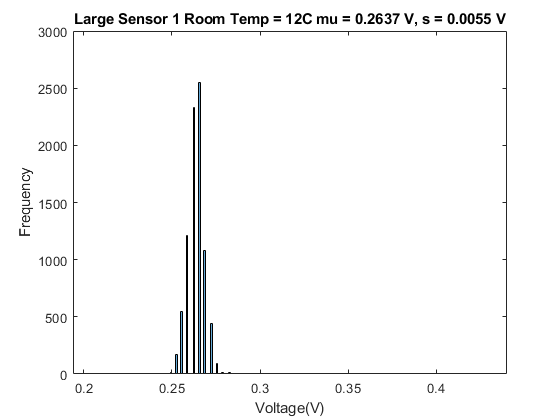
\includegraphics[width=1\linewidth, height=6cm]{Images/Large1RoomHist.png}
    \caption{Large sensor 1 Room Temp Histogram}
    \label{fig:Large1RoomHist}
\end{subfigure}
\begin{subfigure}{0.5\textwidth}
    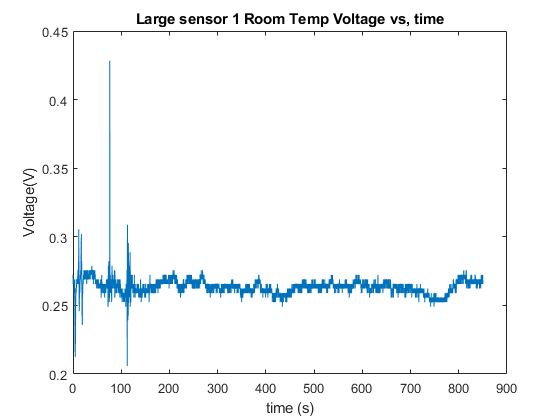
\includegraphics[width=1\linewidth, height=6cm]{Images/Large1RoomTime.png}
    \caption{Large 1 Room temp Voltage vs. Time}
    \label{fig:Large1RoomTime}
\end{subfigure}
\caption{Large Sensor 1 room temperature calibration point}
\label{largeSensor1Room }
\end{figure}

The next data point was the temperature with the hair dryer. This method produced temperatures of 30\textcelsius{}. The time graph and the histogram of values are shown in figure \ref{fig:Large1DryerTime} and figure \ref{fig:Large1DryerHist} respectively.

\begin{figure}[h!]
\begin{subfigure}{0.5\textwidth}
    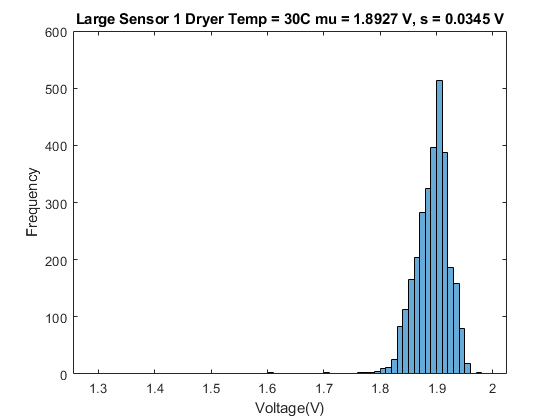
\includegraphics[width=1\linewidth, height=6cm]{Images/Large1DryerHist.png}
    \caption{Large sensor 1 Dryer Temp Histogram}
    \label{fig:Large1DryerHist}
\end{subfigure}
\begin{subfigure}{0.5\textwidth}
    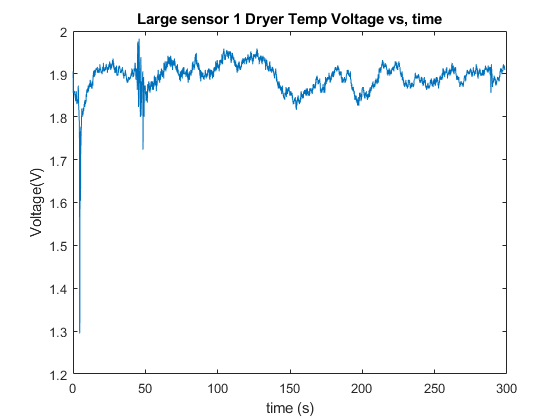
\includegraphics[width=1\linewidth, height=6cm]{Images/Large1DryerTime.png}
    \caption{Large 1 Dryer temp Voltage vs. Time}
    \label{fig:Large1DryerTime}
\end{subfigure}
\caption{Large Sensor 1 dryer temperature calibration point}
\label{largeSensor1Dryer}
\end{figure}

Since all eight of the sensors were calibrated in this fashion, showing detailed plots of all of them would be too cumbersome. So the data has been arranged in table \ref{tab:CalibrationTable}.

\begin{table}[h!]
    \centering
    \caption{Table of Calibration Values}
    \label{tab:CalibrationTable}
    \begin{tabular}{|c|c|c|c|c|c|c|c|}
        \hline
        & Sensors & Room(V) & $\Delta_{Room}$ & $T_{Room}$(C) & Dryer(V) & $\Delta_{Dryer}$ & $T_{Dryer}$(C)   \\
        \hline
        \multirow{4}{*}{Small} & 1 & 0.338 & 0.019 & 12 & 2.179 & 0.058 & 31 \\
        & 2 & 0.332 & 0.021 & 12 & 2.391 & 0.135 & 30 \\
        & 3 & 0.258 & 0.025 & 12 & 2.732 & 0.097 & 30 \\
        & 4 & 0.264 & 0.029 & 12 & 2.501 & 0.095 & 29 \\
        \hline
        \multirow{4}{*}{Large}& 1 & 0.264 & 0.006 & 12 & 1.893 & 0.035 & 30 \\
        & 2 & 0.270 & 0.011 & 11 & 2.003 & 0.107 & 30 \\
        & 3 & 0.252 & 0.011 & 11 & 1.839 & 0.144 & 33 \\
        & 4 & 0.263 & 0.018 & 11 & 1.587 & 0.224 & 33 \\
        \hline
    \end{tabular}
\end{table}

Each sensor is labeled from their respective groups. The Voltage and error($\Delta$) is listed for the given temperature. The measured temperature of the calibration thermometer is also displayed. Since looking at a table is cluttered. The data has been arranged in a calibration plot shown in figure \ref{fig:CalibrationPlot}. The data has been separated into large sensors and small sensors.

\begin{figure}[h!]
    \centering
    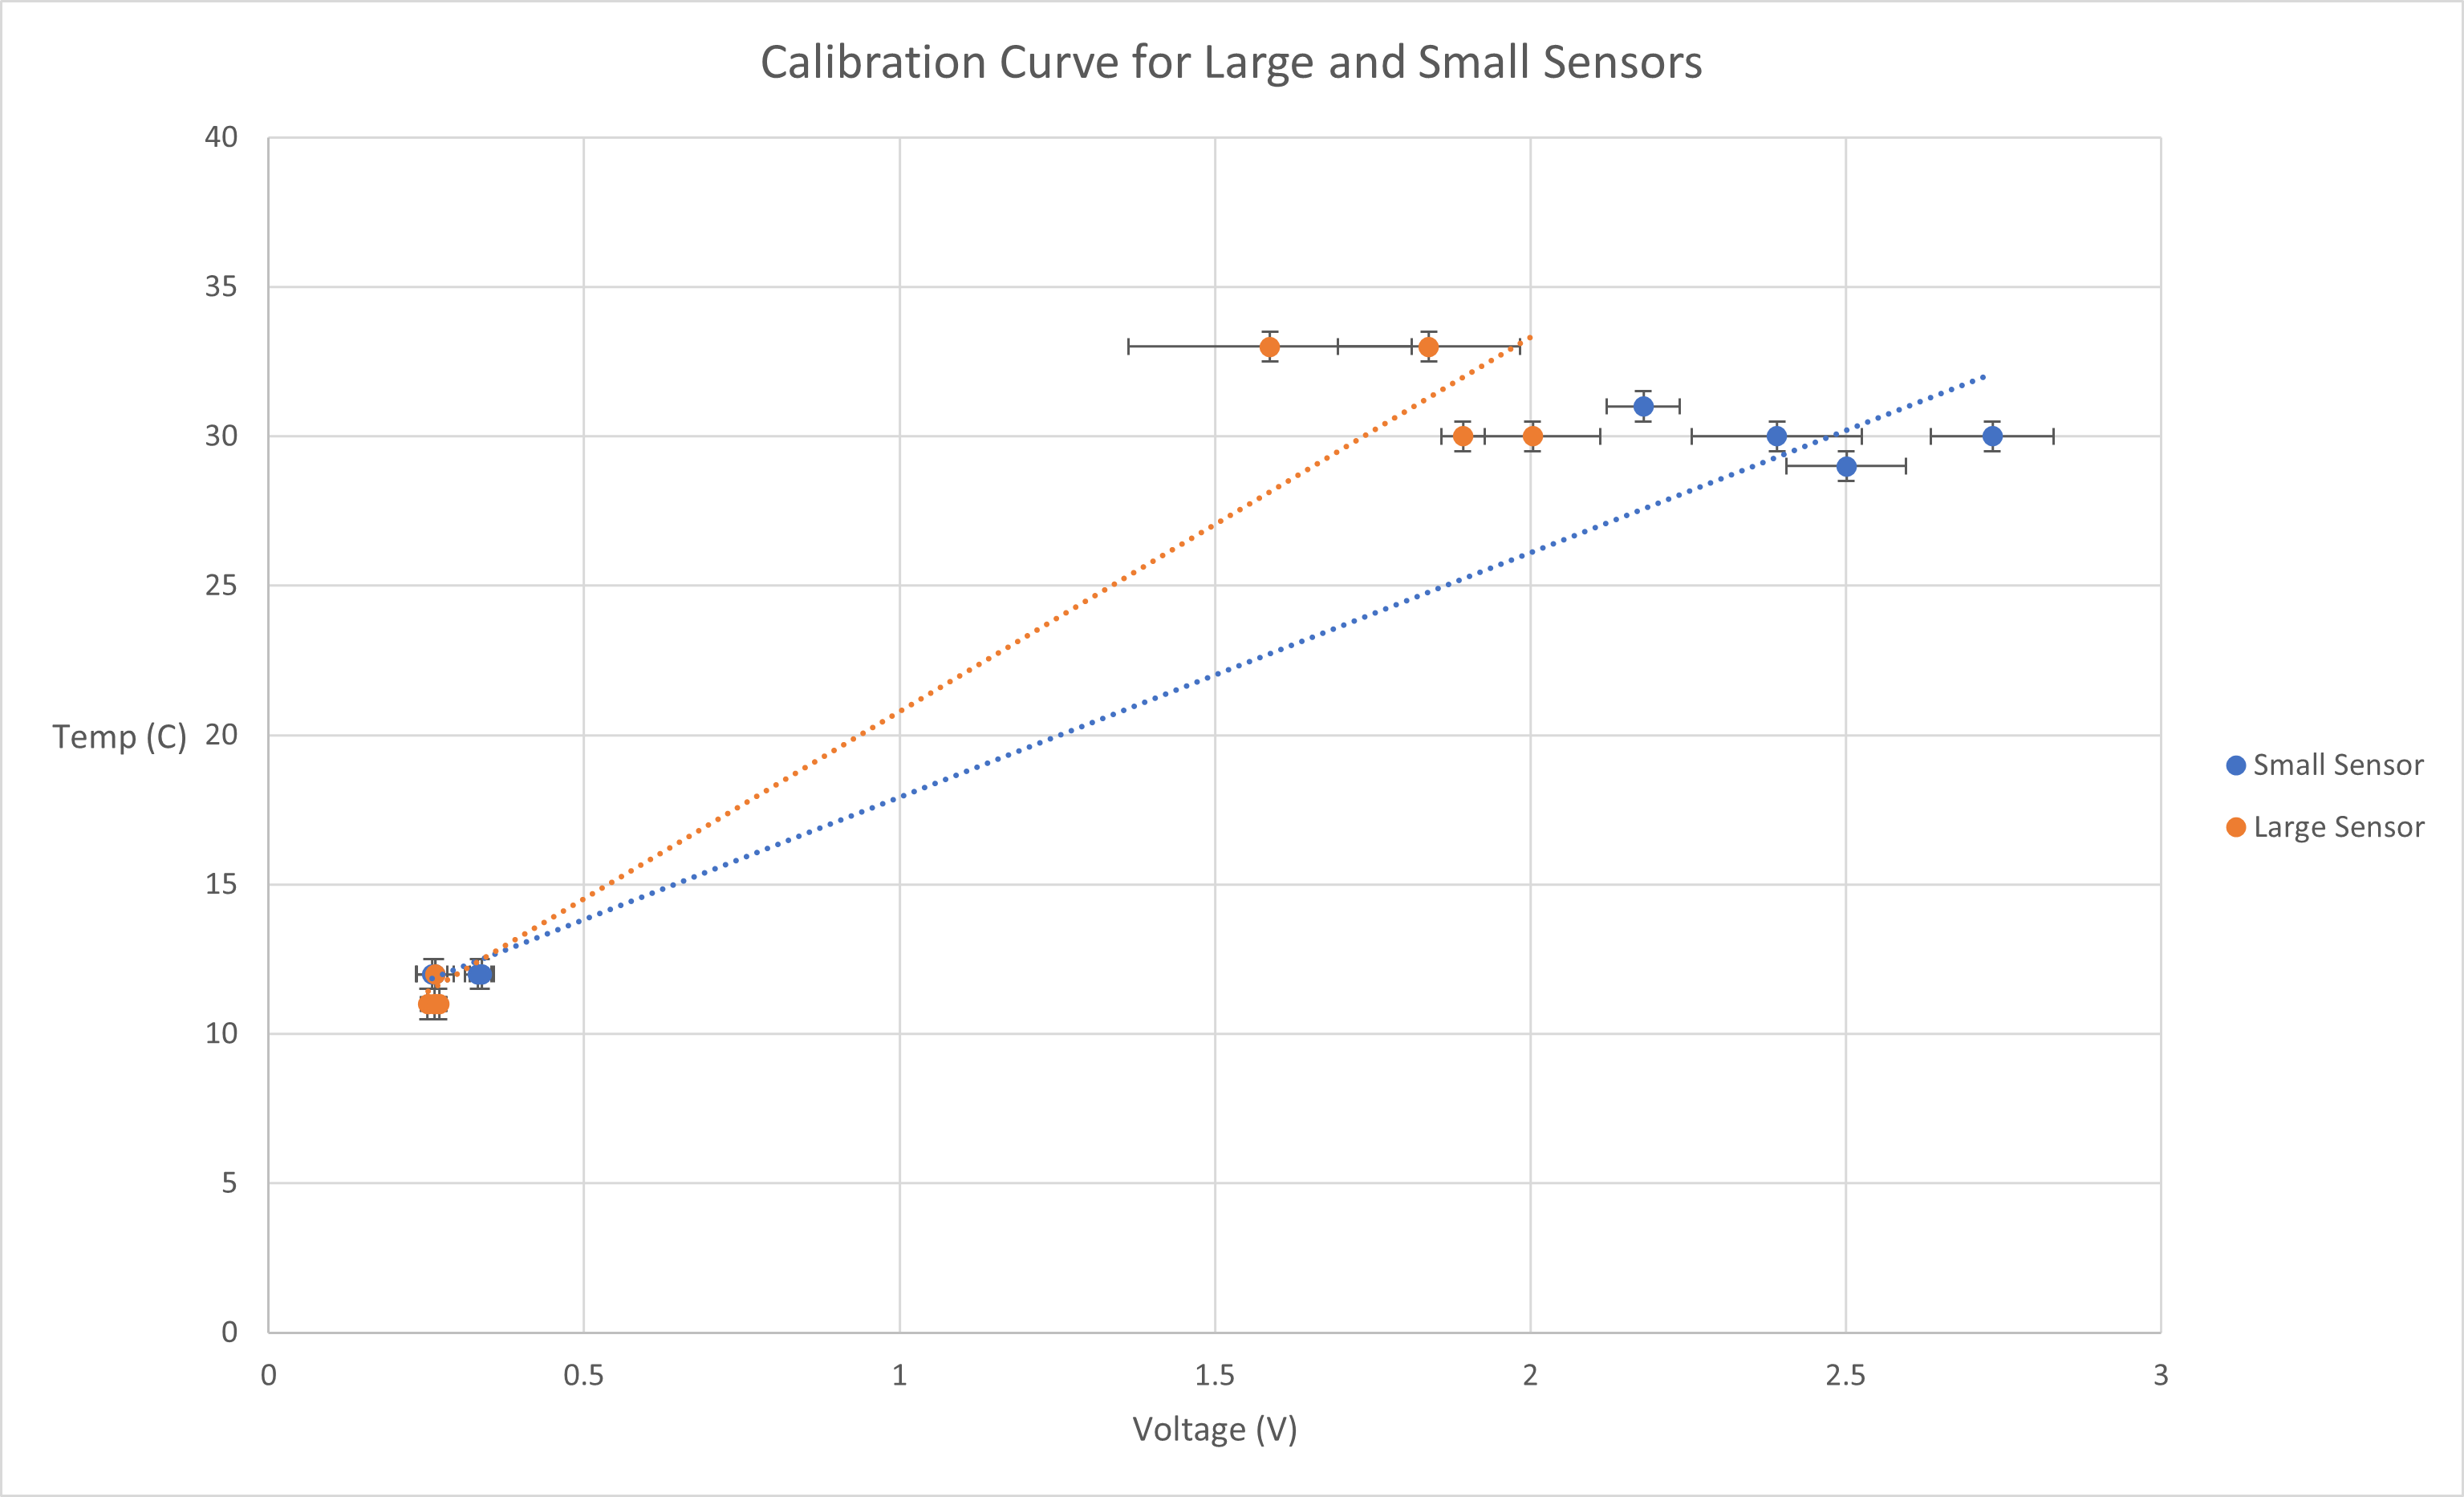
\includegraphics[height = 3in]{Images/Calibration Curve.png}
    \caption{Calibration Values displayed on a graph. There are trend lines that show the line of best for for large and small sensors as a group.}
    \label{fig:CalibrationPlot}
\end{figure}

Something to note about this data is that the large sensors appear to be less sensitive to changes in ambient temperature. That is to say that for a given temperature increase, the larger sensors produce less of a voltage change. This may be caused by the larger silicon chip. In this scenario the silicon chip would act as a larger thermal reservoir and absorb more thermal energy from the thermistor. This means that a sacrifice in the temporal resolution would be the cost of the greater accuracy presumed to be a feature of the larger thermistor.\par





\subsection{Evaluation \& Discussion}

These calibration points were then hard coded into the Arduino IDE and the temperatures of two points on the body were measured, the Wrist and the underarm(body). Figure \ref{fig:Large1wristTime} shows the calibrated temperature vs time of the wrist being measured. notice there are some spikes in this data caused by some shuffling around. The outliers weren't enough to effect the histogram and parameter extraction from Gaussian fitting as shown in figure \ref{fig:Large1wristHist}.

\begin{figure}[h!]
\begin{subfigure}{0.5\textwidth}
    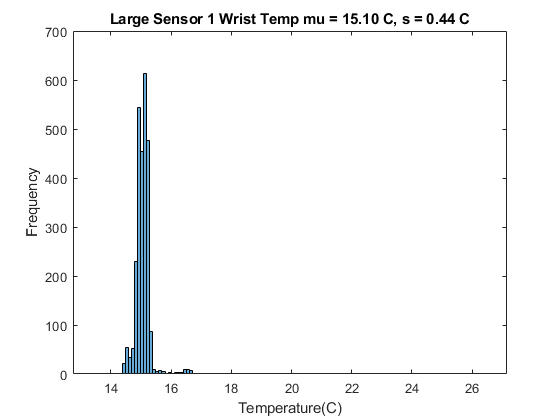
\includegraphics[width=1\linewidth, height=6cm]{Images/Large1WristHist.png}
    \caption{Large sensor 1 wrist temp histogram}
    \label{fig:Large1wristHist}
\end{subfigure}
\begin{subfigure}{0.5\textwidth}
    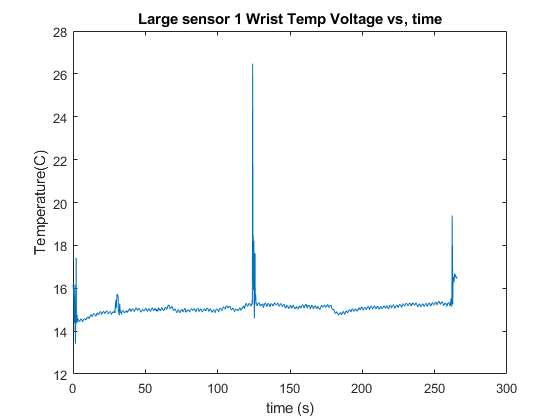
\includegraphics[width=1\linewidth, height=6cm]{Images/Large1WristTime.png}
    \caption{Large 1 wrist Temp vs. Time}
    \label{fig:Large1wristTime}
\end{subfigure}
\caption{Large sensor 1 wrist temperature measurement data}
\label{LargeSensor1Wrist }
\end{figure}

The body temperature was also measured in the underarm. Once again the temporal temperature response and the histogram of temperature values are shown in figure \ref{fig:Large1bodyTime} and figure \ref{fig:Large1bodyHist} respectively. 

\begin{figure}[h!]
\begin{subfigure}{0.5\textwidth}
    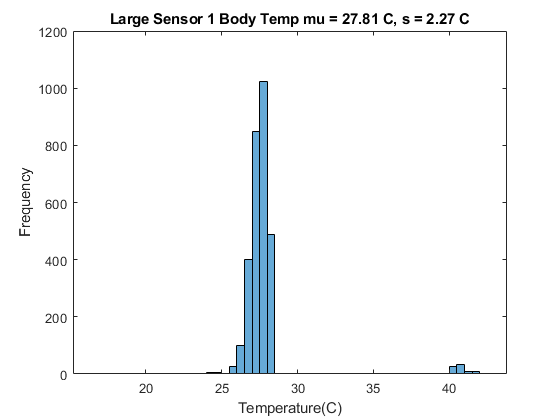
\includegraphics[width=1\linewidth, height=6cm]{Images/Large1ArmHist.png}
    \caption{Large sensor 1 body temp histogram}
    \label{fig:Large1bodyHist}
\end{subfigure}
\begin{subfigure}{0.5\textwidth}
    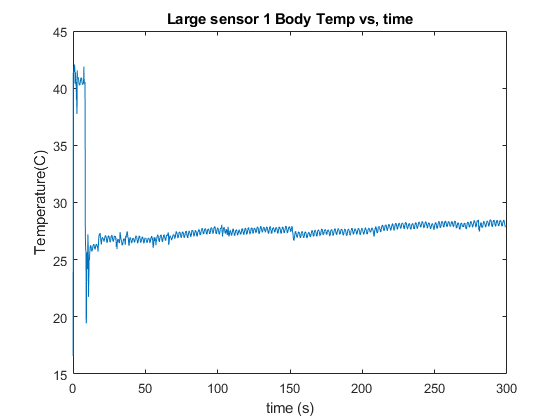
\includegraphics[width=1\linewidth, height=6cm]{Images/Large1ArmTime.png}
    \caption{Large 1 body temp vs. time}
    \label{fig:Large1bodyTime}
\end{subfigure}
\caption{Large Sensor 1 body temperature measurement data}
\label{LargeSensor1Body}
\end{figure}

Notice again the disturbances shown in figure \ref{fig:Large1bodyTime} as there was some motion before settling down for the data collection period. These readings were done with all of the sensors and the data was put into table \ref{tab:MeasuredResults} for easier viewing.

\begin{table}[h!]
    \centering
    \caption{Measured Results for Wrist and Body Temperature}
    \label{tab:MeasuredResults}
    \begin{tabular}{|c|c|c|c|c|c|}
        \hline
        & Sensors & Wrist(C) & $\Delta_{Wrist}$ & Body(C) & $\Delta_{Body}$   \\
        \hline
        \multirow{4}{*}{Small} & 1 & 16.56 & 0.15 & 32.69 & 1.94 \\
        & 2 & 16.55 & 0.57 & 17.18 & 0.81 \\
        & 3 & 15.91 & 0.55 & 17.94 & 0.68 \\
        & 4 & 15.25 & 0.32 & 17.53 & 0.32 \\
        \hline
        \multirow{4}{*}{Large}& 1 & 15.10 & 0.44 & 27.81 & 2.27\\
        & 2 & 13.65 & 0.58 & 23.60 & 0.74 \\
        & 3 & 27.11 & 3.01 & 23.69 & 2.09 \\
        & 4 & 29.15 & 2.19 & 29.58 & 0.56 \\
        \hline
    \end{tabular}
\end{table}

Just like in the calibration table, the small and large sensors were separated and each individual sensor was measured according to their calibration data. The Temperature and error($\Delta$) can be seen for both the wrist and the body for all sensors. This data was then put together into a plot shown in figure \ref{fig:ResultsPlot} to show their positions graphically relative to each other. 

\begin{figure}[h!]
    \centering
    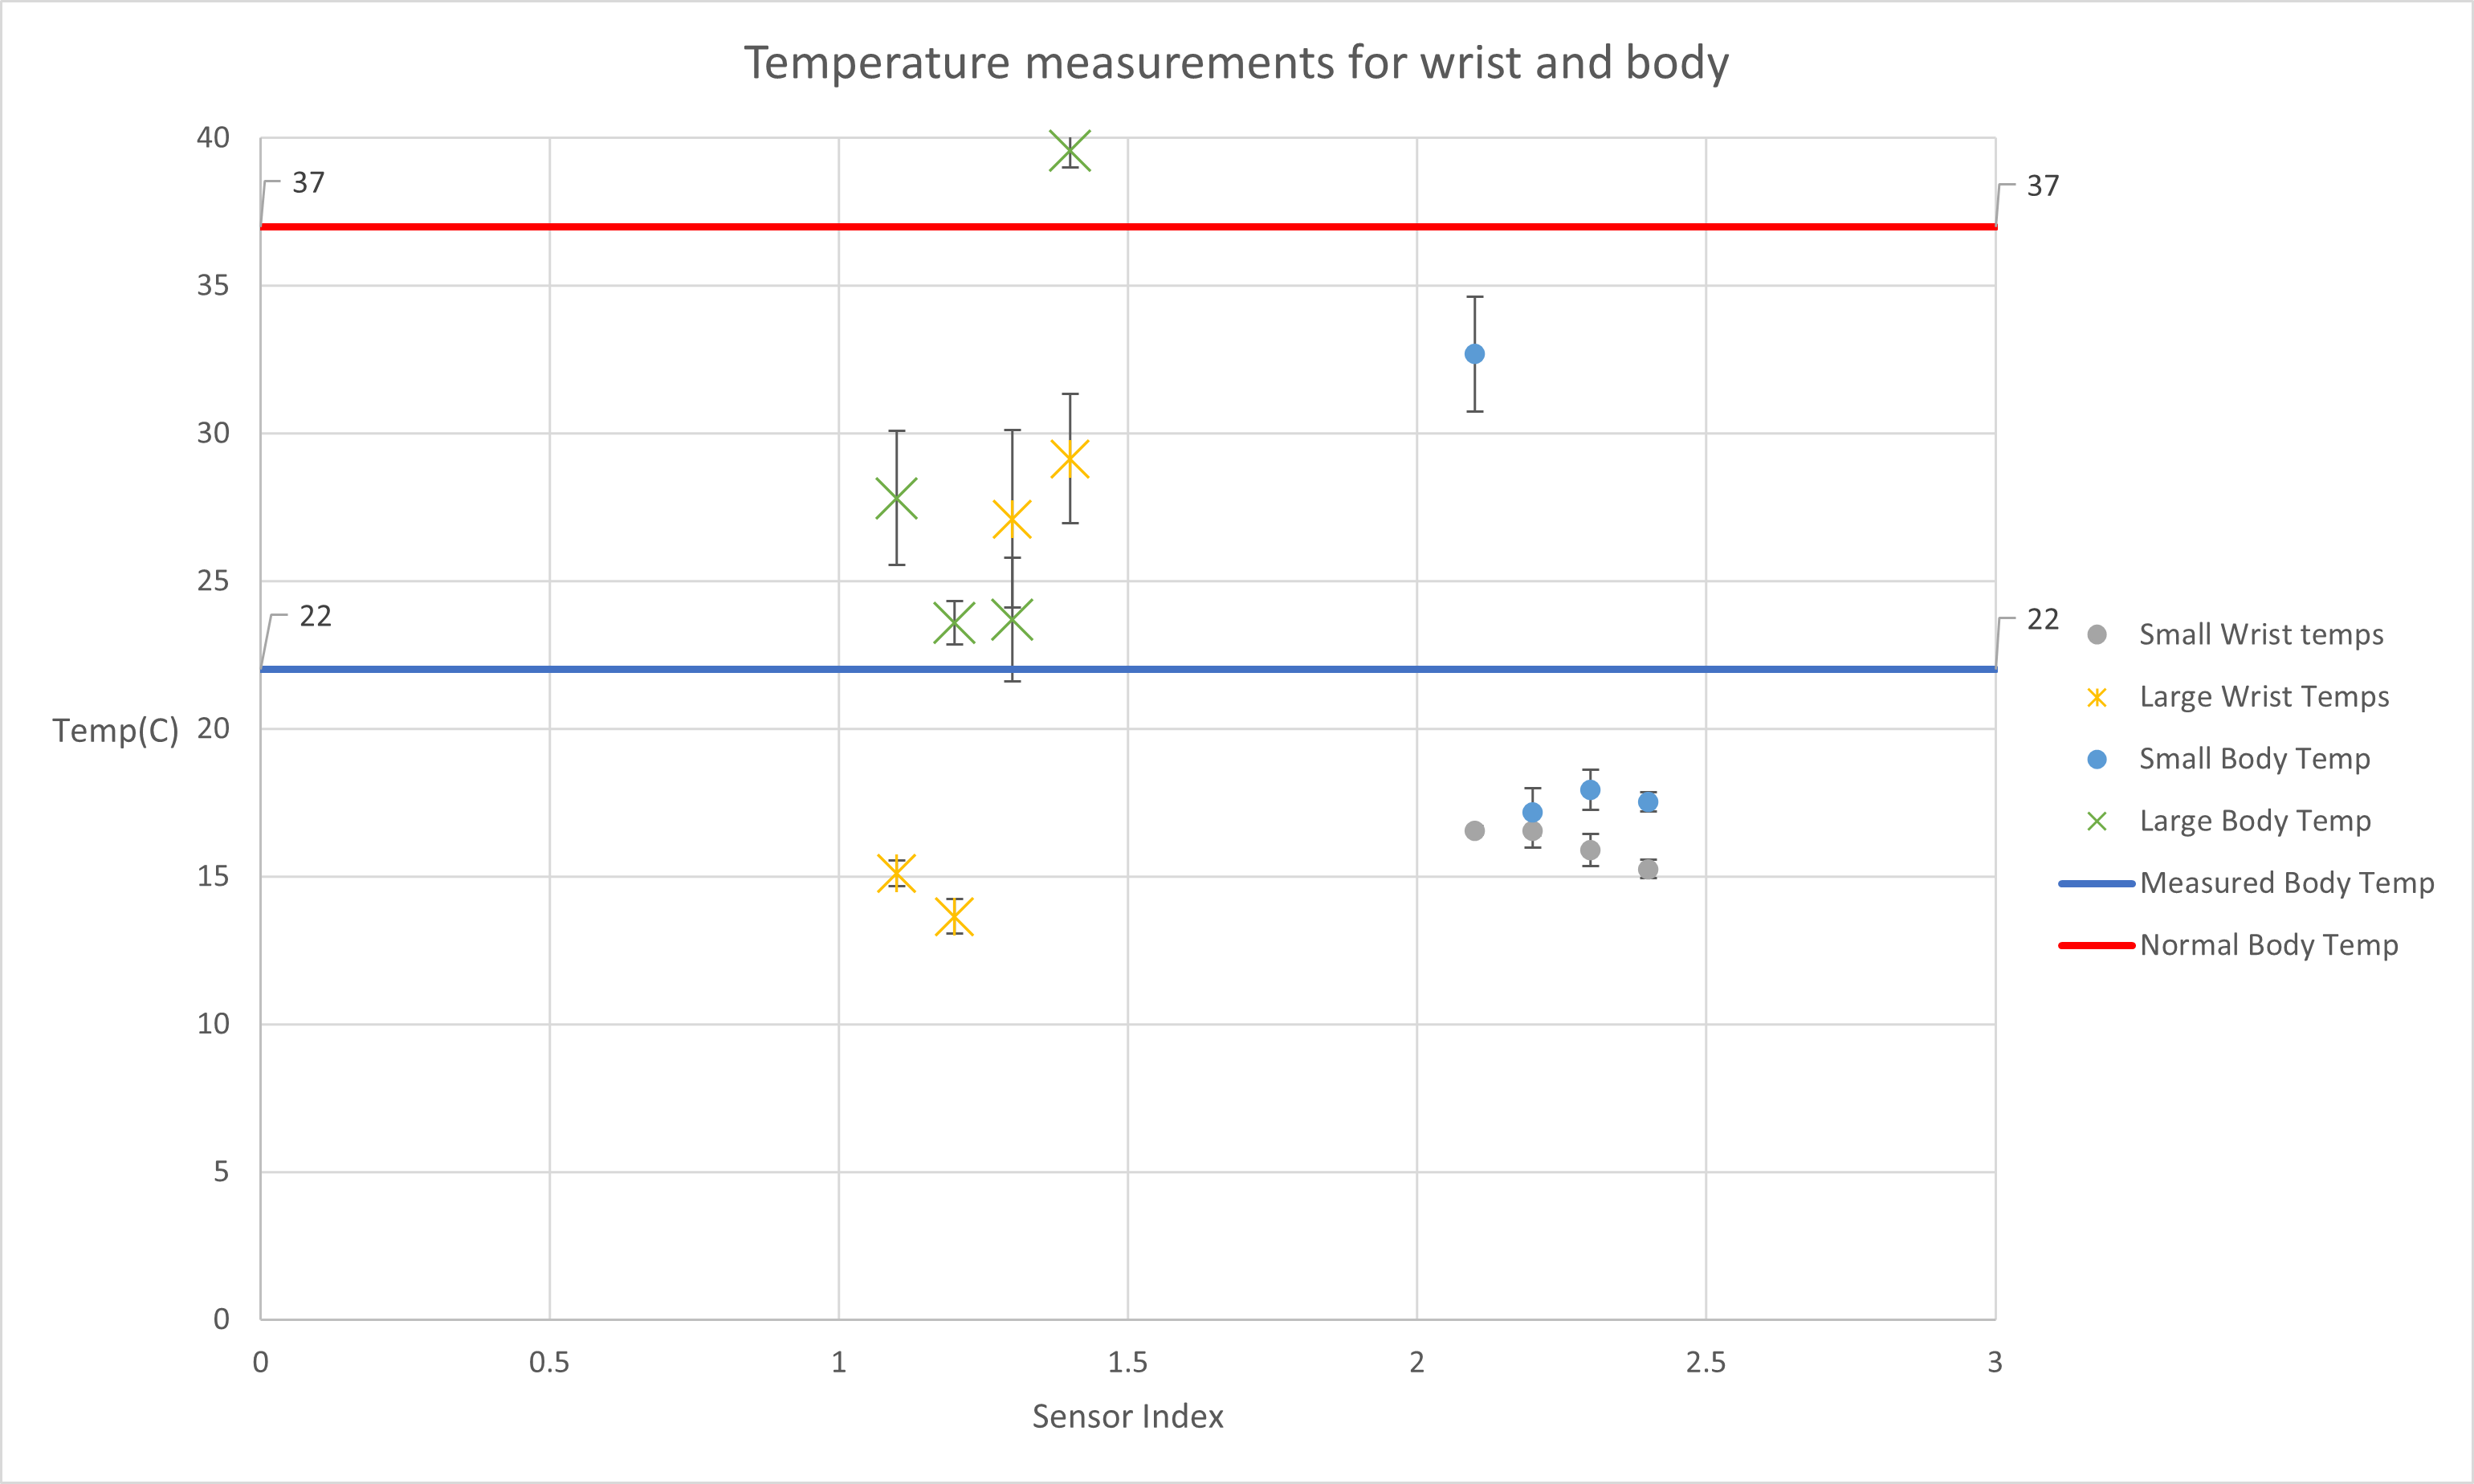
\includegraphics[height = 3in]{Images/Results.png}
    \caption{Results of table \ref{tab:MeasuredResults} displayed on a graph with reference lines for body actual body temperature and body temperature measured from calibration thermometer}
    \label{fig:ResultsPlot}
\end{figure}

Note that there are two horizontal lines in this plot. The bottom line (22\textcelsius{}) represents the temperature of the body as measured by the calibration thermometer. The upper line (37\textcelsius{}) represents the temperature that Google says is the normal body temperature. The bottom axis in figure \ref{fig:ResultsPlot} only serves as an index axis to separate each of the sensors individually and into a group. The large sensors are shown in the left cluster and the small sensors are shown in the right cluster. The height of each point indicates the relevant temperature reading.\par

This plot shows that most of the sensors readings were clustered around where the calibration thermometer measured the body temperature With that in consideration one could say that these sensors are true to their calibration and that there is a systemic error of approximately 15\textcelsius{} in these sensors.


%%%%%%%%%%%%%%%%%%%%%%%%%%%%%%%%%%%%%%%%%%%%%%%%%%%%%%%%%%%%%
\newpage
\section{Conclusion}
%%%%%%%%%%%%%%%%%%%%%%%%%%%%%%%%%%%%%%%%%%%%%%%%%%%%%%%%%%%%%
To conclude the project report I will summarize the main successes and talk about the practical use of the sensors as they ended up. I will talk about the instructions on how to use the sensors and also address any future work that could be completed for this project.


\subsection{Summary}

The project started off with the designing a thermal sensor using resources provided by the professor. The sensor design was then sent to Cameron who designed the mask in L-edit with the help from grad students. The mask ended up being delayed and the fabrication of the sensors was delayed. At the beginning of march the sensors were finalized and delivered to us where I calibrated and then tested the sensors before sending the equipment over to Thomas who when proceeded to test his sensors. The thermal sensors ended up being precise to within a half a degree but there was systemic error was large at 15\textcelsius{}. 


\subsection{Design Implementation and Practical Use}

The sensor requires a conditioning circuit so in order to mass manufacture this it will need to be created with a task specific manufacturing device with the resistors planned out for operational amplifier. The sensor itself would need to be manufactured on Kapton to be flexible and not succumb to the thermal sink the silicon wafer. I also believe that the sensor should be smaller even at the cost of accuracy. The temporal resolution and physical size of the sensor are inappropriate for a bio-metric sensor

\subsection{Instructions for Using the Produced Design}

One sensor at a time needs to be assembled in a circuit as seen in figure \ref{fig:ConditioningCircuit} with the voltage divider resistor of approximately equal value. The circuit takes a voltage of 5V such that the Op-amps can produce the 3.3V needed for the maximum FLORA signal. The potentiometer should be adjusted such that the serial readout of the FLORA is approximately 100 at 12\textcelsius{}. Then the calibration must be hard coded into the FLORA's code. The serial readout will now read the calibrated temperature for the specific sensor that is being used. 

\subsection{Concluding Remarks and Future Work}

Over the course of this project I have thought about how it could be applied to my future career. I am disappointed that I did not get to explore this topic with the help of professor Prakash more in depth as I think that sensor design and implementation is a field in which I would like to work. COVID has undoubtedly effected the lives of many people all over the world, and even today it is still causing problems in the form of new and dangerous variants. The time delays from this virus meant that I did not get to redesign the sensors at all. I also was not able to fabricate the sensors to Kapton or use our own surface mount components to create our own fully wearable flexible sensor node that would transmit data to your phone. I believe this would have been possible if we were allowed to work together at the school, Most of the group seemed motivated to get their work done on this project.\par

For future work, if I had more time, I would have like to preform a redesign of the thermal sensors and fabricated an array of different sizes of sensors. I would have also made the gaps between the sensor wires larger to avoid any kind of field effect resistive properties. These are the two parameters I would have tried to vary in the second redesign.\par

I look forward to applying the lessons that I learned in this project to my future career.






\end{document}
